%--------------------------------------------------------------
%Preamble
%\documentclass[a4paper, twoside, 11pt]{book}
\documentclass[oneside,openany,11pt]{book}
\usepackage[%
  papersize={210mm,297mm},%
  layoutsize={200mm,290mm},%
  layoutoffset=5mm,%
  %twoside,%
  nomarginpar,%
  inner=30mm,%
  outer=20mm,%
  vmargin=23mm,%
  voffset=0mm,
  head=20mm,%
  headsep=10mm,%
  %includefoot,
  foot=5mm,%
  %includefoot,
  %showcrop,%
  %showframe,%
]{geometry}
\setlength{\parindent}{0mm}
\setlength{\parskip}{1mm plus 0.5mm minus 0.5mm}
\setlength{\topskip}{5mm}
\setlength{\textfloatsep}{4mm}
\usepackage{setspace}
\usepackage[pdftex, final]{graphicx}
\graphicspath{{./pics/}}
\usepackage[parfill]{parskip}
\usepackage[margin=1cm]{caption}
\usepackage{microtype}
\usepackage{amssymb}
\usepackage{amsmath}
\usepackage{mathtools}
\usepackage{bm}
\usepackage{tensor}
\usepackage{titlesec}
\usepackage[toc]{appendix}
%\newcommand{\sectionbreak}{\clearpage}
\usepackage[linesnumbered,lined,boxed,commentsnumbered,ruled]{algorithm2e}
\setcounter{tocdepth}{6}
\setcounter{secnumdepth}{6}
%\setcounter{chapter}{1}
%\usepackage{enumitem}
%\setlist{nosep} % or \setlist{noitemsep} to leave space around whole list
\usepackage{graphicx}
\usepackage{subfigure}
%filepath for figures
\graphicspath{{./figures/}}
%tikz
\usepackage{tikz,tikz-3dplot} 
%\usetikzlibrary{calc}
\tdplotsetmaincoords{60}{-25}
\usepackage{verbatim}
\usepackage{amsmath}
\DeclareMathOperator*{\argmin}{arg\,min}
\usetikzlibrary{arrows,positioning} 
\tikzset{
    %Define standard arrow tip
    >=stealth',
    %Define style for boxes
    punkt/.style={
           rectangle,
           rounded corners,
           draw=black, very thick,
           text width=6.5em,
           minimum height=2em,
           text centered},
    % Define arrow style
    pil/.style={
           ->,
           thick,
           shorten <=2pt,
           shorten >=2pt,}
}

\linespread{1.5}

%--------------------------------------------------------------

\begin{document}

%TITLEPAGE
\newgeometry{margin=20mm}
\begin{titlepage}
\title{
	\large
		\textbf{Australian National University}\\[0.5cm]
		\textbf{ENGN4718}\\
	 	\textbf{Engineering Research and Development Project}\\
	 	\textbf{2016}\\[2cm]
	\huge
		\textbf{Rigid Body State Estimation From Sparse Range Measurements}\\[2cm]}
\author{
	\large
		\textbf{Montiel Abello}\\
		\textbf{u5162235}}
\date{
	\large
		\vspace{1cm}
		\textbf{Supervised by Dr Jochen Trumpf and Dr Viorela Ila}}
\maketitle
\end{titlepage}
\restoregeometry

%FRONTMATTER
\frontmatter
\chapter*{Acknowledgements}
\addcontentsline{toc}{chapter}{Acknowledgments}

\chapter*{Abstract}
\addcontentsline{toc}{chapter}{Abstract}
\vspace{-1em}
This thesis concerns mobile robot localisation and mapping through the use of the Extended Kalman Filter (EKF). An EKF is used to integrate an Inertial Navigation System and a Global Satellite Navigation system. The computational requirements of the EKF are reduced using with a compressed design. Simulations using simulated and real data are conducted to test the accuracy, robustness and computational efficiency of the designs.

\markboth{Contents}{Contents}
\tableofcontents
%\input{glossary}
\listoffigures
\chapter*{Aims and Contributions}
\addcontentsline{toc}{chapter}{Aims and Contributions}

Aims: start new research, exploratory\\
Outcomes:
-observer design\\
-simulation toolbox for scanning laser range-finder and rigid bodies.
-noise model for Hokuyo UBG-04LX-F01 - more complete model (combines effect of range, angle) in conditions tested than existing literature
Contributions: used Viorela's functions for conversions between rotation representations. Did everything else

%CHAPTERS
\mainmatter
\chapter{Introduction}

Advances in manufacturing and hardware design have made mobile robots more accessible - not only for research and industrial purposes, but to the general public. However, autonomous robots have largely been limited to indoor, carefully controlled environments. Dense sensors such as light field cameras are becoming cheaper and lighter, promising to allow autonomous robots to acquire detailed measurements of complex environments. To fully utilise the potential of these advancing technologies,  improvements in observer design are required to generate more accurate and detailed descriptions of these environments from dense measurements.

One method of estimating the state of an complex environment is with an infinite-dimensional observer. Typically, observers for infinite-dimensional systems are extensions of finite dimensional Luenberger observers. Unfortunately, this design approach is only able to guarantee convergence for linear systems. Developing a theory of symmetry-preserving, infinite-dimensional observers would simplify the design process for nonlinear systems and result in observers with improved convergence properties.

This research project ...
RESEARCH GOALS\\
	Exploratory, look into sparse sensor - dense measurements. Build an observer for an infinite dimensional system - in this case, simplified at first. Will explore if infinite dimensional, symmetry preserving implementation would improve performance
WHAT IS IN REPORT\\
	This report presents the implementation of an observer to solve a novel problem: estimating cube state from sparse range measurements.
	Simulation - to test performance, experimental validation
	
	implementation of an observer to solve novel problem - sparse sensor gives dense measurement.
	Sparse measurements from a range sensor
	dense measurement part of new direction of research into infinite dimensional symmetry preserving observers.
	Section \ref{sec:literature} reviews literature infinite dimensional observers. Looks at methods for design.
	Relevant background for ... symmetry, state representation. Lie groups. 
	Present problem - detailed breakdown, how it fits into lit. 
	Detailed description of simulation implementation including observer update function design.
	Chapter 
	experimental data - noise model + measurements collected

\section{Literature Review}
\textbf{should this be a chapter???}

Use dense sensors to estimate infinite dimensional state of environment can be achieved through an infinite dimensional observer. Richer theory can be gained by taking advantage of symmetries of the system. Will review progress in infinite dimensional, symmetry preserving observers.

\subsection{infinite-dimensional observers}
In many real world systems the dependent variables are functions of one or more spatial variables. These spatial variables form a continuum of ??? which means an infinite number of parameters are required to describe the state. Such systems are termed infinite dimensional systems, or distributed parameter systems. Their dynamics are modelled by a partial differential equation (PDE). When a state estimate is required but direct measurement of the state with sensors is difficult or impossible, a state observer is employed. A state observer estimates the state of a system using the difference between measured and predicted outputs of the system.

\textbf{linear:}\\
Observer theory for infinite dimensional \textit{linear} systems has been widely studied. The techniques used are typically extensions of Luenberger observers and Kalman filter methods used to observe finite dimensional systems.

A simplified approach is to use a spatial discretisation method such as finite difference or finite element to reduce the infinite dimensional system to a finite dimensional one. From here, finite dimensional observer design techniques can be used. This is known as the early lumping method, and was employed by Stavroulakis \cite{stavroulakis1973design} who implemented a finite dimensional observer as part of a control system for an infinite dimensional systems.

The early lumping approach suffers from \textit{spillover}, a phenomenon where performance is affected by the neglected dynamics \cite{meirovitch1983problem}. Harkort \cite{harkort2011finite} recently developed an observer based control scheme that reduced this effect by using modelled outputs rather than true measurements to reduce the effect of the neglected dynamics.

More accurate observers can be designed with the late lumping approach which uses the infinite dimensional model of the system in the observer design itself. The result is what is an actual infinite dimensional observer that is discretised later for practical implementation. These methods are typically extensions of Kalman or Luenberger observers. 
Gressang \cite{gressang1975observers} extended the Luenberger observer to infinite dimensional systems whose state space was an abstract Banach space - dynamics defined by infinitesimal generator - sort of like basis ? of semigroup.

Smyshlyaev \cite{smyshlyaev2005backstepping} developed an exponentially converging backstepping observer for systems governed by parabolic PDEs.

Ramdani introduced forward and backward observers \cite{ramdani2010recovering}.

Haine \cite{haine2014recovering} applied Ramdani's method, studied convergence properties.

\textbf{nonlinear}

-no universal approach for observer design for infinite-dimensional nonlinear systems\\
-some methods for special case - infinite dimensional bilinear systems. \cite{xu1995observer,bounit1997observers}
-for finite-dimensional nonlinear systems, common design methods are: linearisation (ie EKF), lyapunov method, sliding mode, high gain

\subsection{symmetry preserving observers}
\subsubsection{early work}
\subsubsection{bonnabel et al}
\subsubsection{trumpf, mahony et al}
\subsubsection{juan's work - in detail}


%\section{Literature Review}
\textbf{should this be a chapter???}

Use dense sensors to estimate infinite dimensional state of environment can be achieved through an infinite dimensional observer. Richer theory can be gained by taking advantage of symmetries of the system. Will review progress in infinite dimensional, symmetry preserving observers.

\subsection{infinite-dimensional observers}
In many real world systems the dependent variables are functions of one or more spatial variables. These spatial variables form a continuum of ??? which means an infinite number of parameters are required to describe the state. Such systems are termed infinite dimensional systems, or distributed parameter systems. Their dynamics are modelled by a partial differential equation (PDE). When a state estimate is required but direct measurement of the state with sensors is difficult or impossible, a state observer is employed. A state observer estimates the state of a system using the difference between measured and predicted outputs of the system.

\textbf{linear:}\\
Observer theory for infinite dimensional \textit{linear} systems has been widely studied. The techniques used are typically extensions of Luenberger observers and Kalman filter methods used to observe finite dimensional systems.

A simplified approach is to use a spatial discretisation method such as finite difference or finite element to reduce the infinite dimensional system to a finite dimensional one. From here, finite dimensional observer design techniques can be used. This is known as the early lumping method, and was employed by Stavroulakis \cite{stavroulakis1973design} who implemented a finite dimensional observer as part of a control system for an infinite dimensional systems.

The early lumping approach suffers from \textit{spillover}, a phenomenon where performance is affected by the neglected dynamics \cite{meirovitch1983problem}. Harkort \cite{harkort2011finite} recently developed an observer based control scheme that reduced this effect by using modelled outputs rather than true measurements to reduce the effect of the neglected dynamics.

More accurate observers can be designed with the late lumping approach which uses the infinite dimensional model of the system in the observer design itself. The result is what is an actual infinite dimensional observer that is discretised later for practical implementation. These methods are typically extensions of Kalman or Luenberger observers. 
Gressang \cite{gressang1975observers} extended the Luenberger observer to infinite dimensional systems whose state space was an abstract Banach space - dynamics defined by infinitesimal generator - sort of like basis ? of semigroup.

Smyshlyaev \cite{smyshlyaev2005backstepping} developed an exponentially converging backstepping observer for systems governed by parabolic PDEs.

Ramdani introduced forward and backward observers \cite{ramdani2010recovering}.

Haine \cite{haine2014recovering} applied Ramdani's method, studied convergence properties.

\textbf{nonlinear}

-no universal approach for observer design for infinite-dimensional nonlinear systems\\
-some methods for special case - infinite dimensional bilinear systems. \cite{xu1995observer,bounit1997observers}
-for finite-dimensional nonlinear systems, common design methods are: linearisation (ie EKF), lyapunov method, sliding mode, high gain

\subsection{symmetry preserving observers}
\subsubsection{early work}
\subsubsection{bonnabel et al}
\subsubsection{trumpf, mahony et al}
\subsubsection{juan's work - in detail}

  \section{Theoretical Background}

\subsection{Rigid Body Kinematics}
	A rigid body is a model of a solid object whose deformation is assumed to be negligible. The distance between every pair of points on the body remains constant. Because such a body does not deform, knowledge of the orientation and position of a single point constitutes knowledge of the position and orientation of all points. The position of the rigid body is thus defined as the position of a single point in the body, most commonly its centre of mass. The orientation can be defined using a set of coordinate axes fixed to the body.
	The theory of Lie groups will be used to describe the kinematics of rigid bodies on this report.
			
	\subsubsection{Lie Groups}		
		A Lie group $\mathbf{G}$ is a group that is also a differentiable manifold.
		As a group, $\mathbf{G}$ is a set of elements and a group operation. This group operation is a binary operation that combines two elements and is denoted by multiplication: $AB$ for $A,B \in \mathbf{G}$. Because it is a group, $\mathbf{G}$ satisfies the 4 group axioms:
		\begin{itemize}
		\item \textbf{Closure:} 
			The group operation
			$\mathbf{G} \times \mathbf{G} \mapsto \mathbf{G}$ 
			is a function that maps elements of $\mathbf{G}$ onto itself;
			$\forall A,B \in \mathbf{G}$, $AB \in \mathbf{G}$.
		\item \textbf{Associativity:} Elements of G are associative under the group operation;
			$\forall A,B,C \in \mathbf{G}$, $(AB)C=A(BC)$.
		\item \textbf{Identity:} There exists an identity element $I \in \mathbf{G}$  such that
			$\forall A \in \mathbf{G}$, $IA = AI = A$.
		\item \textbf{Inverse:} For all $A \in \mathbf{G}$ there exists an inverse element $A^{-1} \in \mathbf{G}$ such that $AA^{-1}=A^{-1}A=I$. 
		\end{itemize}
		
		Because the Lie group $\mathbf{G}$ is a differentiable manifold, it is locally Euclidean. This means that the neighbourhood around every element of $\mathbf{G}$ can be approximated with a tangent plane. This property allows calculus to be performed on elements of $\mathbf{G}$.
		
		\textbf{Matrix Lie groups}\\
			A matrix Lie group $\mathbf{G} \in \mathbf{GL}(n)$ is made up of group elements which are $n \times n$ matrices.
			This work will focus on matrix Lie groups because the exponential map and Lie bracket functions given below only apply to such Lie groups.
		
		\textbf{Lie algebra}\\
			The tangent space at the identity element of a Lie group is called the Lie algebra $\mathfrak{g}$. It is called the Lie \textit{algebra} because it has a binary operation, known as the Lie bracket $[X,Y]$. For matrix Lie groups the Lie bracket is
			\begin{equation}
				[A,B] \stackrel{\Delta}{=} AB-BA
			\end{equation}
			
		\textbf{The exponential map and logarithm map}\\		
			The mapping from the Lie algebra $\mathfrak{g}$ to the Lie group $\mathbf{G}$ is called the exponential map:
			\begin{equation}
				\exp: \mathfrak{g} \rightarrow \mathbf{G}
			\end{equation}			
			Similarly, the logarithm map maps elements from $\mathbf{G}$ to $\mathfrak{g}$:
			\begin{equation}
				\log: \mathbf{G} \rightarrow \mathfrak{g}
			\end{equation}
			For matrix Lie groups, the exponential map and logarithm map correspond to matrix exponential and matrix logarithm respectively.
						
		\textbf{Infinitesimal generators}\\
			For an \textit{n}-dimensional matrix Lie group, the Lie algebra $\mathfrak{g}$ is a vector space isomorphic to $\mathbb{R}^n$. The hat operator $\hat{\:}$ maps vectors $x \in \mathbb{R}^3$ to elements of $\mathfrak{g}$.				
			\begin{equation}
				\hat{\:}: x \in \mathbb{R}^n \rightarrow \hat{x} \in \mathfrak{g}
			\end{equation}		
			For a matrix Lie group $\mathbf{G}$ whose elements are $\textit{n} \times \textit{n}$ matrices, the elements of $\mathfrak{g}$ will also be $\textit{n} \times \textit{n}$ matrices. The hat operator is defined
			\begin{equation}
				\hat{x} = \sum\limits_{i=1}^n x_iG^i 
			\end{equation}
			where $G^i$ are $\textit{n} \times \textit{n}$ matrices known as the infinitesimal generators of $\mathbf{G}$.
						
		\textbf{Lie bracket and group operation}\\					
			For Lie groups endowned with the commutative property ($\forall A,B \in \mathbf{G}, AB = BA$), vector addition in the Lie algebra maps to a group operation in the Lie group. For $C = A + B$ where $A,B,C \in \mathfrak{g}$,
			\begin{equation}
				e^C = e^{A+B} = e^Ae^B
			\end{equation}
			For non-commutative Lie groups, the relationship between the Lie bracket and group operation does not hold. Instead, for $C = \log{e^Ae^B}$, $C$ is calculated with the Baker-Campbell-Hausdorff formula:
			\begin{equation}
				C = A + B + \frac{1}{2}[A,B] + \frac{1}{12}[A-B,[A,B]] + \frac{1}{24}[B,[A,[A,B]]] + \dots
			\end{equation}	
		
		\textbf{Actions}\\
			When a group action for a Lie group G acting on a manifold $M$ is a differentiable map, this is known as a Lie group action. For example, 3D rotations act on 3D points so the Lie group $\mathbf{SO}(3)$ acts on $\mathbb{R}^3$. A left action of $\mathbf{G}$ on $M$ is defined as a differentiable map
			\begin{equation}
				\Phi: \mathbf{G} \times M \mapsto M
			\end{equation}
			where
			\begin{itemize}
			\item the identity element $I$ maps M onto itself *(is that the right wording?)
				\begin{equation}
					\Phi(I,m) = m \textnormal{, } \forall m \in M
				\end{equation}
			\item Group actions compose according to
				\begin{equation}
					\Phi(m,\Phi(n,o)) = \Phi(mn,o)
				\end{equation}
			\end{itemize}
			
		\textbf{Adjoint map}\\		
		EXPLANATION???\\
		For $A \in \mathbf{G}$ and $B \in ?$ define a function $\Psi$, known as the adjoint map of $\mathbf{G}$:
		\begin{equation}
			\Psi_A: \mathbf{G} \rightarrow \mathbf{G} \textnormal{, }
			\Psi_A(B) \stackrel{\Delta}{=} ABA^{-1}
		\end{equation}
		Taking the derivative:
		\begin{equation}
			\frac{\partial}{\partial t} \Psi_A(B(t))|_{t=0} = AVA^{-1} \textnormal{, }
			V \stackrel{\Delta}{=} 	\frac{\partial}{\partial t}B(t)|_{t=0}
		\end{equation}
		The adjoint	representation of $\mathbf{G}$ is given by the mapping
		\begin{equation}
			\textbf{Adj}_A: \mathfrak{g} \rightarrow \mathfrak{g} \textnormal{, }
			\textbf{Adj}_A(V) \stackrel{\Delta}{=} AVA^{-1}
		\end{equation}
	
		
	\subsubsection{\textbf{SO}(3)}	
		A rotation represents the motion of a point about the origin of a Euclidean space. In $\mathbb{R}^3$ this is a proper isometry: a transformation that preserves distances between any pair of points and has a determinant of +1. The set of all rotations about the origin of $\mathbb{R}^3$ is known as the \textit{special orthogonal group} $\textbf{SO}(3)$.
		Group elements of $\textbf{SO}(3)$ can be represented using a special subset of $3 \times 3$ invertible matrices and in this case, forms a matrix Lie group. Several rotation representations are described in REF, but the theory presented below only applies to matrix Lie groups which rely on the rotation matrix representation for group elements.
		
		\textbf{Lie algebra}\\
		The Lie algebra $\mathfrak{so}(3)$ is vector space whose elements correspond to an angular velocity. These elements can be represented with $3 \times 3$ skew-symmetric matrices $[\bm{\omega}]_{\times}$, where $\bm{\omega}$ is a 3-vector representing an angular velocity.
		Elements of $\mathfrak{so}(3)$ are mapped to $\textbf{SO}(3)$ according to the exponential map:
		\begin{equation}
			\begin{split}
				\exp: \mathfrak{so}(3) \rightarrow \mathbf{SO}(3)\\
				[\bm{\omega}]_\times \rightarrow \mathbf{R}_{3x3}
			\end{split}		
		\end{equation}		
		i.e. $\forall \omega \in \mathfrak{so}(3) \textnormal{, } \exp([\omega]_\times) \in  \mathbf{SO}(3)$
		
		Conversely, the logarithm map maps $3 \times 3$ rotation matrices of $\mathbf{SO}(3)$ to elements of $\mathfrak{so}(3)$:
		\begin{equation}
			\begin{split}
				\log: \mathbf{SO}(3) \rightarrow \mathfrak{so}(3)\\
				 \mathbf{R}_{3x3} \rightarrow [\bm{\omega}]_\times
			\end{split}		
		\end{equation}		
		i.e. $\forall \mathbf{R} \in \mathbf{SO}(3)  \textnormal{, } \log(\mathbf{R}) \in  \mathfrak{so}(3)$
				
		\textbf{Actions}\\
		By the group action, elements of $\mathbf{SO}(3)$ rotate points in $\mathbb{R}^3$ about the origin. 
		\begin{equation}
			\Phi: \mathbf{SO}(3) \times \mathbf{R}^3 \mapsto \mathbf{R}^3
		\end{equation}
		
		\textbf{Adjoint map}\\
		EXPLANATION???? Hard to explain practical application without discussing reference frames: ie if position defined in body fixed frame but some other transformation defined in inertial frame. First undo rotation to get pose in inertial frame, apply transformation, then re-apply rotation.
		\begin{equation}
			\Psi_R: \mathbf{SO}(3) \rightarrow \mathbf{SO}(3) \textnormal{, }
			\Psi_R(A) \stackrel{\Delta}{=} RAR^{-1}
		\end{equation}
		Taking the derivative:
		\begin{equation}
			\frac{\partial}{\partial t} \Psi_R(A(t))|_{t=0} = RBR^{-1} \textnormal{, }
			B \stackrel{\Delta}{=} 	\frac{\partial}{\partial t}A(t)|_{t=0}
		\end{equation}
		The adjoint	representation of $\mathbf{SO}(3)$ is given by the mapping
		\begin{equation}
			\textbf{Adj}_R: \mathfrak{so}(3) \rightarrow \mathfrak{so}(3) \textnormal{, }
			\textbf{Adj}_R(B) \stackrel{\Delta}{=} RBR^{-1}
		\end{equation}
		
		\textbf{Rotation representations}\\		
		There are many conventions by which elements of $\mathbf{SO}(3)$ can be represented. The representations that will be used in this report are described below.
		
		\textbf{Rotation matrices}\\
		A 3D rotation matrix $\mathbf{R}$ is an orthogonal $3 \times 3$ matrix with a determinant of +1. Since $\mathbf{R}$ is orthogonal, its columns and rows are respectively sets of orthogonal unit vectors and
		\begin{equation}
			\mathbf{R}^{-1} = \mathbf{R}^{T}
		\end{equation}		
		The group operation using rotation matrices is simply a matrix multiplication which concatenates the two rotations. The product of two rotation matrices $\mathbf{R}_3 = \mathbf{R}_2\mathbf{R}_1$ is a rotation matrix corresponding to left multiplication by $\mathbf{R}_1$ followed by $\mathbf{R}_2$.
		
		The left action of a rotation matrix $\mathbf{R}$ on a point $\mathbf{p} \in \mathbb{R}^3$ is a left matrix multiplication that rotates $\mathbf{p}$ about the origin.
		
		\textbf{Scaled-axis representation}\\
		An orientation in $\mathbf{R}^3$ can also be represented by a 3-vector $\bm{\theta}$ whose direction $\mathbf{r}$ represents the axis of rotation and magnitude $\theta$ represents the angle of rotation.
		\begin{equation}
			\bm{\theta} = \theta\mathbf{r}
		\end{equation}
		
		Though scaled-axis vectors are not typically used to perform rotations, Rodrigues' rotation formula efficiently converts scaled-axis vectors to rotation matrices:
		\begin{equation}
			\mathbf{R}_{\bm{\theta}} = \mathbf{I} + [\mathbf{r}]_{\times}\sin{\theta} + ([\mathbf{r}]_{\times})^2(1-\cos{\theta})
		\end{equation}
					
		Elements of $\mathfrak{so}(3)$ are typically represented with a scaled-axis vector $\bm{\omega}$ where the magnitude $|\bm{\omega}|$ corresponds to the angular velocity about the axis $\bm{\omega}/|\bm{\omega}|$.
					
		\textbf{Rotation quaternions}\\
		Quaternions are an extension of complex numbers. The set of unit quaternions can be used to represent $\mathbf{SO}(3)$, and will be referred to as rotation quaternions. 
		A rotation quaternion $\mathbf{q}$ is a 4-tuple of real numbers that encode the same information as axis angle. $\mathbf{q}$ is often described in terms of its first element $w$ - the scalar part, and the remaining elements $x,y$ and $z$ - the vector part. Given an axis of rotation $\mathbf{r}$ and an angle of rotation $\theta$:
		\begin{equation}
			\mathbf{q} = 
			\begin{bmatrix}
				w \\
				x \\
				y \\
				z
			\end{bmatrix}
			 = 
			 \begin{bmatrix}
 				w \\
 				\mathbf{v}
			 \end{bmatrix}
			 =
			 \begin{bmatrix}
			 	\cos(\theta/2) \\
			 	\sin(\theta/2)\mathbf{r}
			 \end{bmatrix}
		\end{equation}
		In general, the quaternion inverse is given by
		\begin{equation}
			\mathbf{q}^{-1} = 
			\frac{1}{w^2 + x^2 + y^2 + z^2}
		 	\begin{bmatrix*}[r]
				 w \\
				-x \\
				-y \\
				-z
			\end{bmatrix*}
		\end{equation}
		For unit magnitude rotation quaternions the inverse represents a rotation by $-\theta$ and is given by
		\begin{equation}
			\mathbf{q}^{-1} = 
			\begin{bmatrix}
			 	\cos(\theta/2) \\
			 	-\sin(\theta/2)\mathbf{r}
		 	\end{bmatrix} =
		 	\begin{bmatrix}
				w \\
				-x \\
				-y \\
				-z
			\end{bmatrix}
		\end{equation}
		
		The group operation is performed with quaternion multiplication which is defined:
		\begin{equation}
			\mathbf{q}_1\mathbf{q}_2 =
			\begin{bmatrix}
			 	w_1 \\
			 	\mathbf{v}_1
			\end{bmatrix} 
			\begin{bmatrix}
			 	w_2 \\
			 	\mathbf{v}_2
			\end{bmatrix} 
			=
			\begin{bmatrix}
			 	w_1w_2 - \mathbf{v}_1 \cdot \mathbf{v}_2 \\
			 	w_1\mathbf{v}_2 + w_2\mathbf{v}_1 + \mathbf{v}_1 \times \mathbf{v}_2
			\end{bmatrix} 
		\end{equation} 
		As with rotation matrices, quaternion multiplication is associative but not commutative.
		
		The group action rotates a point $\mathbf{p} \in \mathbb{R}^3$  to $\mathbf{p}'$ by embedding it as the vector part of a quaternion and using a conjugation operation with $\mathbf{q}$:
		formula for rotating vector:
		\begin{equation}
			\begin{bmatrix}
			 	0\\
			 	\mathbf{p'}
			\end{bmatrix}
			= \mathbf{q}
			\begin{bmatrix}
			 	0\\
			 	\mathbf{p}
			\end{bmatrix}
			\mathbf{q}^{-1}
		\end{equation}
		
	\subsubsection{\textbf{SE}(3)}	
		The special Euclidean group $\textbf{SE}(3)$ represents rigid transformation in $\mathbb{R}^3$. This is a matrix Lie group whose elements are the set of all rigid transformations in $\mathbb{R}^3$ and can be represented with $4 \times 4$ matrices of the form
		\begin{equation}
			\textbf{X} = 
			\begin{bmatrix}
				  \mathbf{R}	&	\mathbf{p} \\
				  \textbf{0}_{1 \times 3}		& 	1 
			\end{bmatrix}
		\end{equation}
		where $\mathbf{R} \in \mathbf{SO}(3)$ and 
		$\mathbf{p} = 
		\begin{bmatrix}
			p_x	& p_y & p_z				
		\end{bmatrix}
		^\top \in \mathbb{R}^3$.
		
		$\textbf{SE}(3)$ is a semidirect product of $\textbf{SO}(3)$ and $ \mathbb{R}^3$. As its group elements contain a rotation matrix and translation vector, $\textbf{SE}(3)$ has 6 degrees of freedom and is a 6-dimensional manifold.
			
		\textbf{Lie algebra}\\
		The Lie algebra $\mathfrak{se}(3)$ is a vector space whose elements are $4 \times 4$ matrices of the form
		\begin{equation}
			\begin{bmatrix}
				  [\mathbf{\omega}]_\times	&  \mathbf{v}\\
				  \textbf{0}_{1 \times 3} & 0						  
			\end{bmatrix}
		\end{equation}
		where $\mathbf{\omega} =
		\begin{bmatrix}
			\omega_x & \omega_y & \omega_z				
		\end{bmatrix}
		^\top \in \mathbf{so}(3)$, representing an angular velocity in scaled axis representation, and
		$\mathbf{v} = 
		\begin{bmatrix}
			v_x & v_y & v_z				
		\end{bmatrix}
		^\top \in T_{\mathbf{p}}\mathbb{R}^3$, representing a linear velocity vector.
		
		Elements of $\mathfrak{se}(3)$ are mapped to $\textbf{SE}(3)$ according to the exponential map:
			\begin{equation}
				\begin{split}
					\exp: \mathfrak{se}(3) \rightarrow \mathbf{SE}(3)\\
					\begin{bmatrix}
						  [\mathbf{\omega}]_\times	&  \mathbf{v}\\
						  \textbf{0}_{1 \times 3} & 0						  
					\end{bmatrix}
					\rightarrow 
					\begin{bmatrix}
						  \mathbf{R}	&	\mathbf{p} \\
						  \textbf{0}_{1 \times 3}		& 	1 
					\end{bmatrix}
				\end{split}		
			\end{equation}		
			i.e. $\forall \mathbf{T} \in \mathfrak{se}(3) \textnormal{, } \exp(\mathbf{T}) \in  \mathbf{SE}(3)$
			
			Conversely, the logarithm map maps elements of $\mathbf{SE}(3)$ to elements of $\mathfrak{se}(3)$:
			\begin{equation}
				\begin{split}
					\log: \mathbf{SE}(3) \rightarrow \mathfrak{se}(3)\\
					\begin{bmatrix}
						\mathbf{R}	&	\mathbf{p} \\
						\textbf{0}_{1 \times 3}		& 	1 					 				  
					\end{bmatrix}
					\rightarrow 
					\begin{bmatrix}
					 	[\mathbf{\omega}]_\times	&  \mathbf{v}\\
					 	\textbf{0}_{1 \times 3} & 0			
					\end{bmatrix}
				\end{split}		
			\end{equation}		
			i.e. $\forall \mathbf{S} \in \mathbf{SE}(3)  \textnormal{, } \log(\mathbf{S}) \in  \mathfrak{se}(3)$
		
		\textbf{Actions}\\
		$\mathbf{SE}(3)$ group elements acts to perform a rigid transformation on points in $\mathbb{R}^3$. This corresponds to a rotation about the origin and a translation.
		To apply a transformation using the $4 \times 4$ matrix elements of $\mathbf{SE}(3)$ to a point $\textbf{p} = (x,y,z) $ in $\mathbb{R}^3$, the point must be represented with homogeneous coordinates: (is $p'$ okay for homogeneous points? $\hat{\:}$ is already used for skew-symmetric matrix)
		\begin{equation}
			\mathbf{p'} = 
			\begin{bmatrix}
				  \mathbf{p} \\
				  1	
			\end{bmatrix} =
			\begin{bmatrix}
				  x	\\
				  y	\\
				  z	\\
				  1	
			\end{bmatrix}
		\end{equation}
		The left group action of $\mathbf{SE}(3)$ is now simply a left matrix multiplication of $\mathbf{p}$:
		\begin{equation}
			\mathbf{p'}_1 = \mathbf{S}\mathbf{p'}_0 = 
			\begin{bmatrix}
				\mathbf{R}	&	\mathbf{p} \\
				\textbf{0}_{1 \times 3}		& 	1 					 				  
			\end{bmatrix}
			\begin{bmatrix}
				\mathbf{p}_0 \\
				1	
			\end{bmatrix}
			=
			\begin{bmatrix}
				\mathbf{R}\mathbf{p}_0 + \mathbf{p}\\
				1	
			\end{bmatrix}
		\end{equation}
				
		\textbf{Adjoint Map}\\
		EXPLANATION\\
		The adjoint map of $\mathbf{SE}(3)$ is
		\begin{equation}
			\Psi_S: \mathbf{SE}(3) \rightarrow \mathbf{SE}(3) \textnormal{, }
			\Psi_S(A) \stackrel{\Delta}{=} SAS^{-1}
		\end{equation}
		Taking the derivative:
		\begin{equation}
			\frac{\partial}{\partial t} \Psi_S(A(t))|_{t=0} = SBS^{-1} \textnormal{, }
			B \stackrel{\Delta}{=} 	\frac{\partial}{\partial t}A(t)|_{t=0}
		\end{equation}
		The adjoint	representation of $\mathbf{SE}(3)$ is given by the mapping
		\begin{equation}
			\textbf{Adj}_S: \mathfrak{se}(3) \rightarrow \mathfrak{se}(3) \textnormal{, }
			\textbf{Adj}_S(B) \stackrel{\Delta}{=} SBS^{-1}
		\end{equation}
		
	\subsubsection{Reference Frames}
		A reference frame is a system of coordinates that is used to uniquely identify points on a manifold. This report will deal with reference frames on $\mathbb{R}^3$, that are used both to define the position of a point and the pose of a rigid body in 3D space.
		Such a reference frame is represented by an element of \textbf{SE}(3).
		
		Consider three different reference frames, denoted \{A\},\{B\} and \{C\}.
		The notation $^{A}_{B}\mathbf{X}^{}_{C}$ defines the transformation in $\mathbf{X}$ of the reference frame \{C\} with respect to the frame \{B\}, defined in the frame \{A\}.
		
		For example, $^{A}_{B}\mathbf{R}^{}_{C}$ defines the rotation of \{C\} with respect to \{B\}, defined in \{A\}.
		
		The notion of an inertial reference frame is introduced here. This will be defined as a reference frame that is stationary for the purpose of the problem being described. 
		
		Figure \ref{fig:frames} shows...
		\begin{figure}
\centering
	\begin{tikzpicture}
		%Frame {A}
		\draw [->](0,0,0)--(1,0,0) node[anchor=west]{$x$};
		\draw [->](0,0,0)--(0,1,0) node[anchor=south]{$y$};
		\draw [->](0,0,0)--(0,0,1) node[anchor=north east]{$z$};
		\node at (0.5,0.5,0) {$\{F\}$};
		%Frame {B}
		\draw [->](8,2,0)--(9,2,1) node[anchor=west]{$x$};
		\draw [->](8,2,0)--(8,3,1) node[anchor=south]{$y$};
		\draw [->](8,2,0)--(8,2,2) node[anchor=north east]{$z$};
		\node at (8.75,2.125,0) {$\{A\}$};
		%Frame {C}
		\draw [->](2,4,0)--(3,3.5,0) node[anchor=west]{$x$};
		\draw [->](2,4,0)--(2.25,5,0) node[anchor=south]{$y$};
		\draw [->](2,4,0)--(2,4,1.5) node[anchor=north east]{$z$};
		\node at (1.5,4.5,0) {$\{B\}$};
		%arrows
		\draw [blue,dashed,->] (0,0,0) to [out=-50, in=-65] (8,2,0);
		\node at (5,-1.5,0) {$^{F}_{F}\mathbf{X}^{}_{A}$};
		\draw [blue,dashed,->] (8,2,0) to [out=50, in=35] (2,4,0);
		\node at (5,5,0) {$^{F}_{A}\mathbf{X}^{}_{B}$};
	\end{tikzpicture}
	  \caption{what frame should transformations be defined in?}
	  \label{fig:frames}
\end{figure}
		
		\textbf{Pose:}\\
		The pose of a rigid body in a given reference frame is defined by its relative position and orientation with respect to the given reference frame and is represented by an element of \textbf{SE}(3). If a rigid body has orientation aligned with a reference frame \{C\} and position at the origin of \{C\}, then the pose of the rigid body with respect to \{B\} and defined in \{A\} is:
		\begin{equation}
			{^{A}_{B}\mathbf{S}^{}_{C}} = 
			\begin{bmatrix}
				^{A}_{B}\mathbf{R}^{}_{C}	& 	^{A}_{B}\mathbf{p}^{}_{C}\\
				\textbf{0}_{1 \times 3} & 1						  
			\end{bmatrix}
		\end{equation}		
		
		\textbf{Point:}\\
		A point $\mathbf{p} \in \mathbb{R}^3$ in the frame \{A\} is denoted $^A\mathbf{p}$ and is expressed as a 3-vector of the weights used to compose it from the basis vectors of \{A\}.
		\begin{equation}
			^{A}\mathbf{p} = 
			\begin{bmatrix}
				^{A}x \\
				^{A}y \\
				^{A}z
			\end{bmatrix}
		\end{equation}
		
		\textbf{Homogeneous coordinates:}\\
		To be acted on by an element of $\mathbf{SE}(3)$, a point must be expressed in homogeneous coordinates:
		\begin{equation}
			^{A}\mathbf{p'} = 
			\begin{bmatrix}
				^{A}\mathbf{p} \\
				1
			\end{bmatrix}
		\end{equation}
		
		\textbf{Defining a point in terms of another reference frame:}\\
		Consider a point in $\mathbb{R}^3$ defined as the position of the frame \{B\} with respect to the frame \{A\}, defined in terms of the frame \{B\}. To redefine the point in terms of \{A\}, the left action of ${^{A}_{A}\mathbf{S}^{}_{B}} \in \mathbf{SE}(3)$ is used:
		\begin{equation}
			^{A}\mathbf{p'} = {^{A}_{A}\mathbf{S}^{}_{B}}\:^{B}\mathbf{p'}
		\end{equation}
		
		\textbf{Concatenating poses:}\\
		Multiply relative poses.
		\begin{equation}
			{^{A}_{A}\mathbf{X}^{}_{C}} = {^{A}_{A}\mathbf{X}^{}_{B}}\:{^{B}_{B}\mathbf{X}^{}_{C}}
		\end{equation}
		
		\textbf{Defining a pose in terms of another reference frame:}\\
		To define a pose transformation matrix in terms of a different reference frame, a matrix conjugation is used:
		\begin{equation}
			{^{B}_{C}\mathbf{X}^{}_{D}} = ({^{B}_{B}\mathbf{X}^{}_{A}})\:{^{A}_{C}\mathbf{X}^{}_{D}}\:({^{B}_{B}\mathbf{X}^{}_{A}})^{-1}
		\end{equation}

		\textbf{Inverse:}\\
		Taking the inverse of a pose transformation matrix has the effect of reversing the transformation, but does not alter the frame that the transformation is defined in terms of.
		\begin{equation}
			({^{A}_{B}\mathbf{X}^{}_{C}})^{-1} = {^{A}_{C}\mathbf{X}^{}_{B}}
		\end{equation}
	
	\subsubsection{Rigid Body State Representation} \label{state rep}
		The state of a rigid body moving through 3D space can be represented by its linear and angular position, velocity and acceleration. Higher derivatives could be taken but will be ignored for simplicity.
		The inertial frame is denoted \{F\} and a frame \{A\} is fixed to the pose of the moving body.
		
		The pose of the body with respect to the inertial frame at time $t$, defined in the inertial frame is represented by the screw matrix ${^{F}_{F}\mathbf{S}^{}_{A}(t)} \in \mathbf{SE}(3)$,
		\begin{equation}
				{^{F}_{F}\mathbf{S}^{}_{A}(t)} = 
				\begin{bmatrix}
						  ^{F}_{F}\mathbf{R}^{}_{A}(t) 	& 	^{F}_{F}\mathbf{p}^{}_{A}(t)\\
						  \textbf{0}_{1 \times 3} & 1						  
				\end{bmatrix}
		\end{equation}
		where $^{F}_{F}\mathbf{R}^{}_{A}(t) \in \mathbf{SO}(3)$ is a rotation matrix, and the position $^{F}_{F}\mathbf{p}^{}_{A}(t) \in \mathbb{R}^3$.
		
		The linear and angular velocity of the body at time $t$ with respect to the inertial frame, defined in the body-fixed frame, is represented by the twist matrix ${^{A}_{F}\mathbf{T}^{}_{A}(t)} \in \mathfrak{se}(3)$,
		\begin{equation}
				{^{A}_{F}\mathbf{T}^{}_{A}(t)} = 
				\begin{bmatrix}
		  {[^{A}_{F}\mathbf{\omega}^{}_{A}(t)]_\times} 	& 	^{A}_{F}\mathbf{v}^{}_{A}(t)\\
		  \textbf{0}_{1 \times 3} & 0						  
				\end{bmatrix}
		\end{equation}
		where $^{A}_{F}\mathbf{\omega}^{}_{A}(t) \in \mathfrak{so}(3)$ is an angular velocity in the scaled-axis representation, and the linear velocity is $^{A}_{F}\mathbf{v}^{}_{A}(t) \in T\mathbb{R}^3$.
				
		The linear and angular acceleration of the body at time $t$ with respect to the inertial frame, defined in the body-fixed frame, is represented by the wrench matrix ${^{A}_{F}\mathbf{W}^{}_{A}(t)} \in T\mathfrak{se}(3)$,
		\begin{equation}
				{^{A}_{F}\mathbf{W}^{}_{A}(t)} = 
				\begin{bmatrix}
				  {[^{A}_{F}\mathbf{\alpha}^{}_{A}(t)]_\times} 	& 	^{A}_{F}\mathbf{a}^{}_{A}(t)\\
				  \textbf{0}_{1 \times 3} & 0						  
				\end{bmatrix}
		\end{equation}
		where $^{A}_{F}\mathbf{\alpha}^{}_{A}(t) \in  T\mathfrak{so}(3)$ is an angular acceleration in the scaled-axis representation, and the linear acceleration is $^{A}_{F}\mathbf{a}^{}_{A}(t) \in T^2\mathbb{R}^3$.
						
		*From now on, will not show frames in notation. This is how S,T,W will be defined unless explicitly stated otherwise.
						
	\subsubsection{Rigid Body Kinematics} \label{kinematics}
		The dynamics of the screw, twist and wrench matrices as they are defined in \ref{state rep} is governed by the following ODEs,
		\begin{equation}
			{\frac{\textnormal{d}}{\textnormal{d}t}} \mathbf{S}(t) =\mathbf{S}(t)\mathbf{T}(t)
		\end{equation}		
		\begin{equation}
			{\frac{\textnormal{d}}{\textnormal{d}t}} \mathbf{T}(t) = \mathbf{W}(t)
		\end{equation}		
		\begin{equation}
			{\frac{\textnormal{d}}{\textnormal{d}t}} \mathbf{W}(t)=\mathbf{f}(t)			
		\end{equation}
		where the function $\mathbf{f}(t)$ is known.
		
	\subsubsection{Scanning Laser Rangefinder Dynamic Model}
		A scanning laser rangefinder fixed to a moving rigid body. State is same as moving rigid body defined above (S,T,W)\\+\\
		Unit vector defined in the body fixed frame  - ${^{A}\mathbf{d}(t)} \in T\mathbb{R}^3$.\\+\\
		Range $r(t) \in \mathbb{R}^{0+}$, defining range from $^{F}_{F}\mathbf{p}^{}_{A}(t)$ to nearest object in environment in direction ${^{F}\mathbf{d}(t)} = {^{F}_{F}\mathbf{R}^{}_{A}(t)}\:{^{A}\mathbf{d}(t)}$
		
		Scan direction in sensor frame is vector rotating at constant speed about $z$-axis, with unit size inside sensor's field-of-view and zero size outside it. Measurements returned at regular, discrete times - when $t$ is an integer multiple of $\delta\tau$:
		\begin{equation}
		^{A}\mathbf{d}(t) =
			\begin{cases} 
			      \hfill \begin{bmatrix}
			      		\cos(-\theta + 2\pi t') \\
			      		-\sin(-\theta + 2\pi t') \\
			      		0
			      	\end{bmatrix}    \hfill & \text{ if $t' \leq \theta/pi$, $t' = k\delta\tau$ where $k \in \mathbb{N}$} \\
			      \hfill \mathbf{0} \hfill & \text{ if $t' > \theta/pi$, $t' \neq k\delta\tau$ where $k \in \mathbb{N}$} \\
			\end{cases} 
		\end{equation}
		where
		\begin{equation}
		t' = \mod(t,1/d\theta)\:d\theta
		\end{equation}
		
		*$\theta_0$ is start of FOV, $t'=X$ at end of FOV

\subsection{Symmetry Preserving Observers}
	\subsubsection{definitions?}
	\subsubsection{construction, ie moving frame method etc}
\subsection{Infinite Dimensional Observers}
\subsection{Discretisation Methods?}
\section{Problem Statement}

\textbf{context:}
Advances in hardware and manufacturing have made autonomous and semi-autonomous robots more available. Use in industry and even general public has increased. Full autonomous robots are still limited to structured environments and tasks such as in factories and warehouses.
Before robots can operate autonomously in unstructured environments, new sensor models are required to more effectively observe and represent complex environment states. \textbf{TODO:} \textit{Why are new sensor models required? Check if this is covered in literature review. If not, need to expand on this.}

\textbf{problem/lacking:}
One method of estimating the state of the environment is to use a state observer. The majority of observer implementations do not take into account the natural symmetries of the dynamics of the state. Doing so has shown to be beneficial in both the design of observers, and improved convergence properties.
However, these invariant observer methods are still limited to finite dimensional systems. In many implementations involving infinite-dimensional systems, the system is discretised to a finite dimensional one prior to observer design.  \textbf{TODO:} \textit{How does this influence performance?}\\
What is needed is a theory of infinite dimensional, symmetry preserving observers, + design principles.

\textbf{what will this theory provide?:}
This theory will simplify invariant observer design for infinite dimensional systems. Only discretising after observer design will maximise the potential of dense sensors. This will allow for more accurate and fast estimation of complex environments,

\textbf{approach:}
This project aims to develop some of this theory. The approach taken will be to design an invariant observer for a specific infinite dimensional system, before generalising the results.

\textbf{estimation problem - cube pose \& size:}
The environment the robot is moving throughout consists of a room (rectangular prism) + cube; each of unknown size and pose.
Attached to the robot is a 2D laser rangefinder. Using depth measurements from this sensor, the observer must estimate the size and pose of the cube. It is assumed that the room is stationary and the cube has constant angular and linear acceleration.\\
\textbf{TODO:} \textit{Diagram}\\
\textbf{TODO:} \textit{Precise mathematical description of problem}

\textbf{deliverables:} 
The primary deliverable of this project is the observer design and simulation. Will later try to develop some general theory from this specific case. Will validate simulation with experiment using Hokuyo UBG 04-LX sensor, ??? robot arms and cubes of various sizes and materials.
\textbf{TODO:} \textit{More detail, + be careful about what you promise}\\


\chapter{Simulation}
\section{Implementation}
A simulation toolbox was implemented in Matlab to model scanning laser range-finder measurements and test observer schemes. The main components of the simulation are:
\begin{itemize}
\item rigid body trajectory computation;
\item solid object modelling;
\item range measurement simulation;
\item noise modelling;
\item observer implementation.
\end{itemize}

A high level description of the simulation is provided in Algorithm \ref{main}.\\
Load settings - saved data can be loaded here\\
Initialise sensor, computes pose of sensor, scan directions over time + creates sensor class instance with sensor settings for noise generation\\
Initialise environment, creates environment class instance - points in body frame, triangles, computes position of points over time\\
Initialise observer - creates observer class instance\\
For each time step, get state of sensor and environment \& compute range - this is done with a parallel for loop\\
Add noise to ranges\\
Observer simulation: each time step, update estimate based on estimated state (kinematics - numerical integration), predict range measurement, check if observing object, if yes update estimate  based on measured and predicted range.

\IncMargin{2em}	
	\begin{algorithm}[H]
	\DontPrintSemicolon
	\SetKwFunction{loadsettings}{loadsettings}
	\SetKwFunction{initialisesensor}{initialisesensor}
	\SetKwFunction{initialiseenvironment}{initialiseenvironment}
	\SetKwFunction{initialiseobserver}{initialiseobserver}
	\SetKwFunction{computerange}{computerange}
	\SetKwFunction{addnoise}{addnoise}
	\SetKwFunction{estimatestate}{estimatestate}
	\SetKwFunction{updatestate}{updatestate}
	\SetKwFunction{identifyobject}{identifyobject}	
	\KwData{\\
	%CHANGE THESE TO LETTERS
	$n_{steps}$ - no. steps in simulation\\
	$\mathbf{X}_s$ - pose and scan direction\\
	$\mathbf{X}_e$ - points for cube and background, triangles\\
	$\hat{\mathbf{X}}_c$ - estimate of pose and size of cube\\
	$c$ - true/false, current range measurement of cube\\
	$\mathbf{r}$ - ground truth range\\
	$\tilde{\mathbf{r}}$ - measured range - ground truth + noise\\
	$\hat{\mathbf{r}}$ - predicted range from state estimate\\
	$\bm{\alpha}$ - angle of incidence for each measurement\\
	$\mathbf{m}$ - index of triangle measured\\
	$\bm{\theta}$ - scan angle in sensor frame\\
	$\bm{\Theta}$ - set of scan angles that return range measurement\\
	}
	\Begin{
		$settings \leftarrow $\loadsettings\\
		$\mathbf{X}_s \leftarrow \initialisesensor(settings)$\\
		$\mathbf{X}_e  \leftarrow \initialiseenvironment(settings)$\\
		\initialiseobserver\\
		\For{$ii \leftarrow 1$ \KwTo $n_{steps}$}{
			\If{$\bm{\theta}[ii] \in \bm{\Theta}$}{
				$[\mathbf{r}[ii],\bm{\alpha}[ii],\mathbf{m}[ii]] \leftarrow \computerange(\mathbf{X}_s[ii],\mathbf{X}_e[ii])$
			}
		}
		$\tilde{\mathbf{r}} = \addnoise(\mathbf{r},\bm{\alpha},\mathbf{m},settings)$\\
		\For{$ii \leftarrow 1$ \KwTo $n_{steps}$}{
			$\hat{\mathbf{X}}_c[ii+1] \leftarrow \estimatestate(\hat{\mathbf{X}}_c[ii])$\\
			\If{$\bm{\theta}[ii] \in \bm{\Theta}$}{
				$\hat{\mathbf{r}}[ii] \leftarrow \computerange(\mathbf{X}_s[ii],\hat{\mathbf{X}}_c[ii])$
				$c \leftarrow \identifyobject(c,\tilde{\mathbf{r}})$\\
				\If{$c$}{
					$\hat{\mathbf{X}}_c[ii+1] \leftarrow \updatestate(\hat{\mathbf{X}}_c[ii+1])$
				}
			}
		}
	}
	\caption{Scanning range-finder and state observer simulation} \label{main}
	\end{algorithm}

\subsection{Rigid Body Motion}
To simulate range measurements the pose of the sensor and the objects comprising the environment must be computed at each time step. The computations required to do so can be reduced by taking into account the kinds of motion that must be simulated.

The observer actually computes the \textit{relative} position between the sensor and cube and simply uses knowledge of the sensor pose to determine the pose of the cube in the inertial frame. There is no need to simulate complex sensor motions because the motion of the cube can be adjusted to achieve the same result. The only requirement of the sensor motion is that a large field of view is acquired so that the entire target object can be viewed. The scanning behaviour of the sensor is to rotate back and forth about the $z$-axis of the body fixed frame $\{A\}$. To provide a rectangular field of view, the motion of the sensor is therefore limited to constant velocity rotation about $y$-axis of inertial frame $\{F\}$.

The environment is modelled with two rigid bodies: a cube to be observed as the target object, and a stationary rectangular prism enclosing the sensor and cube acting as the background. The various cube motions that will be simulated to test the observer's performance can be classed in terms of the wrench matrix of the cube as either
\begin{enumerate}
\item ${\textbf{W}_c} = \textbf{0}$
\item ${\textbf{W}_c} \neq \textbf{0}$
\end{enumerate}

For case 1. the wrench and screw are constant so only the initial value is required. It is more efficient to represent the pose of a rigid body with just position and orientation in this case. The pose can be quickly computed by interpolating between an initial and final pose. For case 2. the screw, twist and wrench must be integrated numerically.

\subsubsection{Interpolation}
To compute a trajectory of $k$ poses beginning at $\{\mathbf{p}_i,\mathbf{q}_i\}$ and ending at $\{\mathbf{p}_f,\mathbf{q}_f\}$:

Poses for each time $\mathbf{t} =
					\begin{bmatrix}
						t_1 & t_2 & t_3 & \dots & t_k
					\end{bmatrix}$

Linear interpolation for position $\mathbf{P}= \begin{bmatrix}
													\mathbf{p}_1 & \mathbf{p}_2 & \mathbf{p}_3 & \dots & \mathbf{p}_k
											   \end{bmatrix}$:
\begin{equation}
	\mathbf{P} = 
	{\mathbf{p}_1}_{[1 \times k]} + (\mathbf{p}_k - \mathbf{p}_1)\frac{\mathbf{t}-{\mathbf{t}_1}_{[1 \times k]}}{t_k - t_1}
\end{equation}
OR?
\begin{equation}
	\mathbf{P} = 
	{\mathbf{P}_1}_{[1 \times k]} + (\mathbf{p}_k - \mathbf{p}_1)\frac{\mathbf{t}-{\mathbf{t}_1}_{[1 \times k]}}{t_k - t_1}
\end{equation}


Spherical linear interpolation for orientation quaternion $\mathbf{q}= \begin{bmatrix}
													\mathbf{q}_1 & \mathbf{q}_2 & \mathbf{q}_3 & \dots & \mathbf{q}_k
												\end{bmatrix}$:

\begin{equation} \label{slerp}
	\mathbf{Q} = \frac{\mathbf{q}_1\sin((\mathbf{1}_{[1 \times k]}-\mathbf{t})\theta) + \mathbf{q}_k\sin(\mathbf{t}\theta)}{\sin(\theta)}
\end{equation}
where
\begin{equation}
	\theta = \cos^{-1}(\mathbf{q}_1 \cdot \mathbf{q}_k)
\end{equation}

*MAKE THESE CLEARER

SCANNING:\\
Require multiple views of target object,reverse trajectory, concatenate and replicate\\
concatenate:\\
\begin{equation}
	\mathbf{P}_{loop}= 
	\begin{bmatrix}
		\mathbf{p}_1 & \mathbf{p}_2 & \mathbf{p}_3 & \dots & \mathbf{p}_k &
		\mathbf{p}_{k} & \mathbf{p}_{k-1} & \mathbf{p}_{k-2} & \dots & \mathbf{p}_1
	\end{bmatrix}
\end{equation}
\begin{equation}
	\mathbf{Q}_{loop}= 
	\begin{bmatrix}
		\mathbf{q}_1 & \mathbf{q}_2 & \mathbf{q}_3 & \dots & \mathbf{q}_k &
		\mathbf{q}_{k} & \mathbf{q}_{k-1} & \mathbf{q}_{k-2} & \dots & \mathbf{q}_1
	\end{bmatrix}
\end{equation}
replicate:
\begin{equation}
	\mathbf{P} = {\mathbf{P}_{loop}}_{[1 \times k]}
\end{equation}
\begin{equation}
	\mathbf{Q} = {\mathbf{Q}_{loop}}_{[1 \times k]}
\end{equation}



\subsubsection{Numerical Integration} \label{integration}
The time evolution of the screw, twist and wrench is computed iteratively from initial conditions by numerically integrating the ODEs in section \ref{kinematics}. For a rigid body with an associated reference frame $\{X\}$:

\begin{equation}
	\mathbf{S}_X(t+\delta t) = \mathbf{S}_X(t)\exp({\delta t {\mathbf{T}_X(t)}})
\end{equation}

\begin{equation}
	\mathbf{T}_X(t+\delta t) = \mathbf{T}_X(t) + \delta t \mathbf{W}_X(t)
\end{equation}

Assuming constant acceleration
\begin{equation}
	\mathbf{W}_X(t+\delta t) =\mathbf{W}_X(t)
\end{equation}

*More accurate integration method not essential - ground truth is ground truth, experimental data won't be nearly as smooth anyway.

In practice, compute orientation quaternion from screw matrix - pose still represented with quaternion and vector - same as interpolation case.

\subsection{Sensor modelling}
The state of the sensor $\mathbf{X}_{s}(t)$ consists of terms corresponding to its motion and scanning operation. 

\subsubsection{Motion}
Since motion restricted, state of sensor actually implemented as 
\begin{equation}
	\mathbf{X}_{s}(t) = \{\mathbf{p}_s(t),\mathbf{q}_s(t),{^{A}\mathbf{s}(t)}\}
\end{equation}

Stationary position:
\begin{equation}
	\mathbf{p}_1 = \mathbf{p}_2 = \mathbf{p}_3 = \dots =  \mathbf{p}_k = 
	\begin{bmatrix}
		0 \\ 0 \\ 0
   	\end{bmatrix}
\end{equation}

													
Rotating from $-\phi$ to $\phi$ about $y$-axis of inertial frame ie interpolate between $\mathbf{q}_1$ and $\mathbf{q}_k$ with equation \ref{slerp}.
	
\begin{equation}
	\mathbf{q}_1 = \begin{bmatrix}
				 	\cos(-\phi/2) \\
				 	\sin(-\phi/2){\begin{bmatrix}
								 	0 \\ 1 \\ 0
							   	 \end{bmatrix}}
				 \end{bmatrix}
				 = \begin{bmatrix}
		 		   		\cos(\phi/2) \\ 0 \\ -\sin(\phi/2) \\ 0
				   \end{bmatrix}
\end{equation}

\begin{equation}
	\mathbf{q}_k = \begin{bmatrix}
				 	\cos(\phi/2) \\
				 	\sin(\phi/2){\begin{bmatrix}
								 	0 \\ 1 \\ 0
							   	 \end{bmatrix}}
				 \end{bmatrix}
				 = \begin{bmatrix}
		 		   		\cos(\phi/2) \\ 0 \\ \sin(\phi/2) \\ 0
				   \end{bmatrix}
\end{equation}

\subsubsection{Scanning}
The scanning behaviour of the sensor is modelled with the vector ${^{A}\mathbf{n}(t)}$.
To simulate a 2D scanning sensor the following parameters are used:
\begin{itemize}
\item field of view $[-\theta,\theta]$: rotation about -z-axis of sensor frame ie anticlockwise about z-axis. in practice, this is represented by start angle, scan direction and field of view angle
\item number of scans $n_{scans}$: number of scan angles in 1 rev. Gives angular resolution $d\theta = \dfrac{2\pi}{n_{scans}}$
\item revolutions per second $\Omega$: This gives each time step as $d\tau = \dfrac{1}{n_{scans}\Omega}$
\end{itemize}
From these parameters, create vector ${^{A}\mathbf{s}(t)}$. At each time $t$, ${^{A}\mathbf{s}(t)}$ is either a unit vector indicating the direction of measurement in the sensor frame, or has $\mathbf{0}$ magnitude the when sensor is not returning a measurement (outside FOV)

scan direction: $^{A}\mathbf{s}(t)$
\begin{equation}
^{A}\mathbf{n}(t) =
	\begin{cases} 
	      \hfill \begin{bmatrix}
	      		\cos(-\theta + 2\pi t') \\
	      		-\sin(-\theta + 2\pi t') \\
	      		0
	      	\end{bmatrix}    \hfill & \text{ if $t' \leq \theta/pi$, $t' = k\delta\tau$ where $k \in \mathbb{N}$} \\
	      \hfill \mathbf{0} \hfill & \text{ if $t' > \theta/pi$, $t' \neq k\delta\tau$ where $k \in \mathbb{N}$} \\
	\end{cases} 
\end{equation}
where
\begin{equation}
t' = \mod(t,1/d\theta)\:d\theta
\end{equation}

*$\theta_0$ is start of FOV, $t'=X$ at end of FOV

Scan direction in inertial frame required for measurement simulation:
\begin{equation}
	{^{F}\mathbf{d'}(t)} = \mathbf{X}_s(t)\:{^{A}\mathbf{d'}(t)}
\end{equation}

\subsection{Environment Modelling}
\subsubsection{Motion}
Pose of object is actually pose of centre of mass of object.
Each object modelled with S. from initial conditions, numerically integrate S,T,W. If constant velocity motion, faster to use waypoints like sensor.
From pose of object at each time, compute pose of all points that make up object: 3D array, each slice is set of points at time ii

\subsubsection{Rigid Objects}
Environment composed of rectangular prisms. These objects are modelled as an ordered set of 8 points in the inertial reference frame, and 12 triangles. Each triangle is a set of 3 integers, indicating the index of the three points that make up its vertexes.
The position (in the inertial frame) of each of these points at each time is determined using the screw matrix and position in body frame (side lengths of the object \& default cube points).

cube points in body frame:
initialPoints = s*0.5*[];
\begin{equation}
	\mathbf{P}_c = \frac{1}{2}s
	\begin{bmatrix*}[r]
		-1  &  -1  &  -1  &  -1  &   1  &   1  &   1  &  1 \\
		-1  &  -1  &   1  &   1  &  -1  &  -1  &   1  &  1 \\
		-1  &   1  &  -1  &   1  &  -1  &   1  &  -1  &  1 
	\end{bmatrix*}
\end{equation}
Shift each according to pose of sensor to get cube points in inertial frame. In sim, rotated with quaternions.
triangles:
\begin{equation}
	\mathbf{T} = 
	\begin{bmatrix}
	1 & 2 & 3 \\
	2 & 4 & 3 \\
    4 & 3 & 7 \\
    4 & 8 & 7 \\
    5 & 6 & 7 \\
    8 & 6 & 7 \\
    2 & 6 & 5 \\
    2 & 1 & 5 \\
    2 & 6 & 8 \\
    2 & 4 & 8 \\
    1 & 5 & 7 \\
    1 & 3 & 7
	\end{bmatrix}
\end{equation}

See figure~\ref{fig:cubeproblem}
\begin{figure}
	\begin{tikzpicture} [scale = 1,tdplot_main_coords] %fix main coords!!!

		%Frame {B}
		\draw [thick,->](0, 0, 0)--(-2, 0, 0) node[anchor=east]{$y$};
		\draw [thick,->](0, 0, 0)--(0, 2, 0) node[anchor=south]{$z$};
		\draw [thick,->](0, 0, 0)--(0, 0, -2) node[anchor=south]{$x$};
		\node at (0.5,1.8,0) {\{F\}};
		%points
		\node[anchor=west] at (-1,-1,-1) {$1$};
		\node[anchor=west] at (-1,-1, 1) {$2$};
		\node[anchor=west] at (-1, 1,-1) {$3$};
		\node[anchor=west] at (-1, 1, 1) {$4$};
		\node[anchor=west] at ( 1,-1,-1) {$5$};
		\node[anchor=west] at ( 1,-1, 1) {$6$};
		\node[anchor=west] at ( 1, 1,-1) {$7$};
		\node[anchor=west] at ( 1, 1, 1) {$8$};
		%cube lines
		\draw (-1,-1,-1)--(-1,-1, 1);   %1-2
		\draw (-1,-1,-1)--(-1, 1,-1);   %1-3
		\draw (-1,-1,-1)--( 1,-1,-1);   %1-5
		\draw (-1,-1, 1)--(-1, 1, 1);   %2-4
		\draw (-1,-1, 1)--( 1,-1, 1);   %2-6	
		\draw (-1, 1,-1)--(-1, 1, 1);   %3-4 	 
		\draw (-1, 1,-1)--( 1, 1,-1);   %3-7	
		\draw (-1, 1, 1)--( 1, 1, 1);   %4-8 
		\draw ( 1,-1,-1)--( 1,-1, 1);   %5-6	
		\draw ( 1,-1,-1)--( 1, 1,-1);   %5-7 
		\draw ( 1,-1, 1)--( 1, 1, 1);   %6-8 
		\draw ( 1, 1,-1)--( 1, 1, 1);   %7-8 
		%triangle lines
		\draw (-1,-1,-1)--(-1, 1, 1);   %1-4
		\draw (-1,-1,-1)--( 1,-1, 1);   %1-6
		\draw (-1,-1,-1)--( 1, 1,-1);   %1-7 
		\draw (-1,-1, 1)--( 1, 1, 1);   %2-8
		\draw (-1, 1,-1)--( 1, 1, 1);   %3-8
		\draw ( 1,-1,-1)--( 1, 1, 1);   %5-8
		
	\end{tikzpicture}
	  \caption{caption}
	  \label{fig:triangles}
\end{figure}





\subsection{Measurement Modelling}
	\subsubsection{Range Computation}
	Given the screw matrix (in the inertial frame) and scan direction (in the body fixed frame) of the sensor, the position and scan direction in the inertial frame are determined.
	The distance to the nearest environment object from this point, along the scan direction is determined with the M{\"o}ller-Trumbore ray-triangle intersection algorithm.
	Difficult to visualise from code, include diagram for case of ray \& single triangle?

	\IncMargin{2em}
	\begin{algorithm}
	\DontPrintSemicolon
	\SetKwInOut{Input}{input}\SetKwInOut{Output}{output}
	\SetKwFunction{size}{size}
	\SetKwFunction{any}{any}
	\SetKwFunction{min}{min}
	\SetKwFunction{find}{find}
	\SetKwFunction{atan}{atan}
	
	\Input{$\mathbf{o}$ - ray origin\\
		   $\mathbf{d}$ - ray direction vector\\
		   $\mathbf{P}$ - cube in inertial frame \\
		   $\mathbf{T}$ - triangle matrix}
	\Output{$x$ - True/False - measurement corresponds to object\\
			$r$ - distance to object in m\\
			$\theta$ - incidence angle in rad\\
			$m$ - index of triangle hit}
	\Begin{
		\tcc{initialise outputs}
		$x \longleftarrow 0$\\
		$r \longleftarrow NaN$\\
		$\theta \longleftarrow NaN$\\
		$m \longleftarrow NaN$\\
		\tcc{triangle vertexes and edges}
		$\mathbf{V}_1 \longleftarrow \mathbf{P}[\mathbf{T}[:,1]]$\\
		$\mathbf{V}_2 \longleftarrow \mathbf{P}[\mathbf{T}[:,2]]$\\
		$\mathbf{V}_3 \longleftarrow \mathbf{P}[\mathbf{T}[:,3]]$\\
		$\mathbf{E}_1 \longleftarrow \mathbf{V}_2 - \mathbf{V}_1$\\
		$\mathbf{E}_2 \longleftarrow \mathbf{V}_3 - \mathbf{V}_1$\\
		$m = \size(\mathbf{V}_1,1)$\\
		$\mathbf{A} \longleftarrow \mathbf{o}_{[m \times 1]} - \mathbf{P}$\\
		\tcc{determinant}
		$\mathbf{B} \longleftarrow \mathbf{d}_{[m \times 1]} \times \mathbf{E}_2$ *(along dim 2)\\
		$\bm{\delta} \longleftarrow \mathbf{E}_1 \cdot \mathbf{B}$ *(along dim 2)\\		
		$\mathbf{y} \longleftarrow |\bm{\delta}|\leq\mathbf{0}$\\
		$\bm{\delta}[\mathbf{y}] \longleftarrow \mathbf{NaN}$\\
		\tcc{barycentric coordinates}
		$\mathbf{u} \longleftarrow (\mathbf{A} \cdot \mathbf{B})/\bm{\delta}$ *(along dim 2)\\
		$\mathbf{Q} \longleftarrow \mathbf{A} \times \mathbf{E}_1$ *(along dim 2)\\
		$\mathbf{v} \longleftarrow (\mathbf{d}_{[n \times 1]} \cdot \mathbf{Q})/\bm{\delta}$ *(along dim 2)\\
		$\mathbf{s} \longleftarrow (\mathbf{E}_2 \cdot \mathbf{Q})/\bm{\delta}$\\
		\tcc{intersection vector}	
		$\mathbf{z} \longleftarrow \mathbf{y} \textbf{ and } (\mathbf{u} \geq \mathbf{0}) 
		\textbf{ and } (\mathbf{v} \geq \mathbf{0}) \textbf{ and } (\mathbf{u}+\mathbf{v} \leq 
		\mathbf{0})$\\
		$\mathbf{x} \longleftarrow \mathbf{z} \textbf{ and } (\mathbf{s} \geq \mathbf{0})$\\
		\If{$\any(\mathbf{x})$}{
			$x \longleftarrow 1$\\
			$\mathbf{x}[\textbf{not }\mathbf{x}] \longleftarrow \mathbf{NaN}$\\
			$\mathbf{r} = \mathbf{s} \circ \mathbf{x}$\\
			$r = \min(\mathbf{r})$\\
			$m = \find(\mathbf{r} = r,1)$\\
			$\mathbf{e}_1 \longleftarrow \mathbf{E}_1[t,:]$\\ 
			$\mathbf{e}_2 \longleftarrow \mathbf{E}_2[t,:]$\\ 
			$\mathbf{n} = \mathbf{e}_1 \times \mathbf{e}_2$\\
			$\theta = \atan(|\mathbf{d}\times\mathbf{n}|,\mathbf{d}\cdot\mathbf{n})$ *atan2\\
			$\theta = \min(\theta,\pi-\theta)$
		}
	}
	\caption{M{\"o}ller-Trumbore ray-triangle intersection\label{MTalg}}
	\end{algorithm}
	
	\subsubsection{Object Surface}
	random walk
	
	\subsubsection{Sensor Noise}
	Noise model depends on sensor used.
	\begin{equation}
		\hat{r}(t) = f_s(r(t),\theta(t),\phi(k))
	\end{equation}
	where $\theta(t)$ is incidence angle of measurement, $\phi$ is surface properties of object $k$ that was measured, $f$ is some function for noise model of particular sensor.
	
	For Hokuyo UBG-04LX-F01 used, noise model was measured experimentally:
	\begin{equation}
		f_{UBG}(r,\theta,\phi) = 
	\end{equation}
	
	
\subsection{Observer implementation}
	\subsubsection{Estimate: internal model}
		The state of the cube at each time step is estimated using the numerical integration method described in section \ref{integration}.
	
	\subsubsection{Identifying object/background}
		The variable \textit{observingObject} indicates whether the range measurement is of the target object or the background. It is assumed that initially the sensor will be observing background, so $\textit{observingObject}_0 = FALSE$

		\textbf{Range assumption:}
		Assuming that the object is within X, background outside
		PSEUDOCODE
		if range $\leq$ X
			c = 1
		else
			c = 0
		end
		
		\textbf{Difference assumption:}
		if $abs(range_{i+1}-range_i) > X$
			c = mod(c+1,2)
		end
		
		\IncMargin{2em}
		\begin{algorithm}
		\DontPrintSemicolon
		\SetKwInOut{Input}{input}\SetKwInOut{Output}{output}
	
		\Input{$rangeAssumption$ - true/false\\
			   $differenceAssumption$ - true/false\\
			   $r_{max}$ - max range for cube\\
			   $\Delta_{max}$ - max diff between measurements of same object\\
			   $c$ - true/false - current measurement is of cube\\
			   $\mathbf{r}_{i+1}$ - distance to object at $t = i+1$\\
			   $\mathbf{r}_{i}$ - distance to object at $t = i$}
		\Output{$c$ - true/false}
		\Begin{				
			\If{$differenceAssumption$}{
				\If{$|\mathbf{r}_{i+1}-\mathbf{r}_{i}| > \Delta_{max}$}{
					$c = \mod(c + 1,2)$
				}
			}
			\If{$rangeAssumption$}{
				\If{$\mathbf{r}_{i+1} > r_{max}$}{
					$c = 0$
				}
			}
		}
		\caption{Target/background object separation}
		\end{algorithm}
		
	\subsubsection{Update}
		\textbf{Input ranges:}\\
			Use ranges according to ordered sequence of indexes $a$. ie if all present - quadrilateral with points at corners:
			\begin{equation}
				a = \{ii,(ii-1),(ii-n_{scans}),(ii-1-n_{scans})\}
			\end{equation}
		
		\textbf{Orientation update:}\\
			Require at least 3 ranges in prediction and measurement. ie
			$|\hat{a}| \geq 3$ and $|\tilde{a}| \geq 3$
	
			From range and direction, compute coordinates of intersection\\
			\begin{equation}
				\mathbf{P}(a_k) = \mathbf{R}(a_k){^{F}\mathbf{N}(a_k)}
			\end{equation}
			\begin{equation}
				\mathbf{n} = [\mathbf{P}(a_2) - \mathbf{P}(a_1)] \times [\mathbf{p}(a_3) - \mathbf{p}(a_1)]
			\end{equation}
			Rotation axis from cross product of predicted and measured normals:\\
			\begin{equation}
				\mathbf{r}_{update} = \hat{\mathbf{n}} \times \tilde{\mathbf{n}}
			\end{equation}
			Rotation angle determined in settings. Table REF shows settings	
			
			figure~\ref{fig:orientation}
			\begin{figure}
	\centering
	\tdplotsetmaincoords{60}{-10}
	\begin{tikzpicture} [scale = 2,tdplot_main_coords] %fix main coords!!!

		%Frame {F}
		\draw [thick,->](0, 0, 0)--(-1, 0, 0) node[anchor=east]{$y$};
		\draw [thick,->](0, 0, 0)--(0, 1, 0) node[anchor=south east]{$x$};
		\draw [thick,->](0, 0, 0)--(0, 0, 1) node[anchor=south]{$z$};
		\node at (0.1,-0.2,0) {\{F\}};

		%ground truth cube lines
		\tdplotsetrotatedcoords{0}{0}{0}
		\coordinate (Shift) at (0,7.5,0);
		\tdplotsetrotatedcoordsorigin{(Shift)}
		\draw [blue,thick,tdplot_rotated_coords] (-1,-1,-1)--(-1,-1, 1);   %1-2
		\draw [blue,thick,tdplot_rotated_coords] (-1,-1,-1)--(-1, 1,-1);   %1-3
		\draw [blue,thick,tdplot_rotated_coords] (-1,-1,-1)--( 1,-1,-1);   %1-5
		\draw [blue,thick,tdplot_rotated_coords] (-1,-1, 1)--(-1, 1, 1);   %2-4
		\draw [blue,thick,tdplot_rotated_coords] (-1,-1, 1)--( 1,-1, 1);   %2-6	
		\draw [blue,thick,tdplot_rotated_coords] (-1, 1,-1)--(-1, 1, 1);   %3-4 	 
		\draw [blue,thick,tdplot_rotated_coords] (-1, 1,-1)--( 1, 1,-1);   %3-7	
		\draw [blue,thick,tdplot_rotated_coords] (-1, 1, 1)--( 1, 1, 1);   %4-8 
		\draw [blue,thick,tdplot_rotated_coords] ( 1,-1,-1)--( 1,-1, 1);   %5-6	
		\draw [blue,thick,tdplot_rotated_coords] ( 1,-1,-1)--( 1, 1,-1);   %5-7 
		\draw [blue,thick,tdplot_rotated_coords] ( 1,-1, 1)--( 1, 1, 1);   %6-8 
		\draw [blue,thick,tdplot_rotated_coords] ( 1, 1,-1)--( 1, 1, 1);   %7-8 
			%normal vector
		\draw [blue,thick,tdplot_rotated_coords,->] (0,-1,0)--(0,-2,0);
		
		%ground truth cube lines
		\tdplotsetrotatedcoords{10}{5}{5}
		\coordinate (Shift) at (0,7.5,0);
		\tdplotsetrotatedcoordsorigin{(Shift)}
		\draw [red,tdplot_rotated_coords] (-1,-1,-1)--(-1,-1, 1);   %1-2
		\draw [red,tdplot_rotated_coords] (-1,-1,-1)--(-1, 1,-1);   %1-3
		\draw [red,tdplot_rotated_coords] (-1,-1,-1)--( 1,-1,-1);   %1-5
		\draw [red,tdplot_rotated_coords] (-1,-1, 1)--(-1, 1, 1);   %2-4
		\draw [red,tdplot_rotated_coords] (-1,-1, 1)--( 1,-1, 1);   %2-6	
		\draw [red,tdplot_rotated_coords] (-1, 1,-1)--(-1, 1, 1);   %3-4 	 
		\draw [red,tdplot_rotated_coords] (-1, 1,-1)--( 1, 1,-1);   %3-7	
		\draw [red,tdplot_rotated_coords] (-1, 1, 1)--( 1, 1, 1);   %4-8 
		\draw [red,tdplot_rotated_coords] ( 1,-1,-1)--( 1,-1, 1);   %5-6	
		\draw [red,tdplot_rotated_coords] ( 1,-1,-1)--( 1, 1,-1);   %5-7 
		\draw [red,tdplot_rotated_coords] ( 1,-1, 1)--( 1, 1, 1);   %6-8 
		\draw [red,tdplot_rotated_coords] ( 1, 1,-1)--( 1, 1, 1);   %7-8 
			%normal vector
		\draw [thick,red,tdplot_rotated_coords,->] (-0.25,-1.1,0)--(-0.25,-2.1,0);
		
		%measurement
		\draw [dashed,black,->] (0,0,0)--(-1*0.6,13*0.6,-0.5*0.6);
		\draw [dashed,black,->] (0,0,0)--(1*0.6,13*0.6,-0.5*0.6);
		\draw [dashed,black,->] (0,0,0)--(0*0.6,13*0.6,1*0.6);
		%ground truth
		\node [draw,blue,circle,inner sep=1pt,fill] at (-0.5, 6.5, -0.25) {};	
		\node [draw,blue,circle,inner sep=1pt,fill] at (0.5, 6.5, -0.25) {};
		\node [draw,blue,circle,inner sep=1pt,fill] at (0, 6.5, 0.5) {};	
		\draw [blue] (-0.5, 6.5, -0.25)--(0.5, 6.5, -0.25);
		\draw [blue] (-0.5, 6.5, -0.25)--(0, 6.5, 0.5);
		\draw [blue] (0, 6.5, 0.5)--(0.5, 6.5, -0.25);
		%prediction
		\node [draw,red,circle,inner sep=1pt,fill] at (-0.5*0.97, 6.5*0.97, -0.25*0.97) {};	
		\node [draw,red,circle,inner sep=1pt,fill] at (0.5*1.03, 6.5*1.03, -0.25*1.03) {};
		\node [draw,red,circle,inner sep=1pt,fill] at (0*0.96, 6.6*0.96, 0.5*0.96) {};	
		\draw [red] (-0.5*0.97, 6.5*0.97, -0.25*0.97)--(0.5*1.03, 6.5*1.03, -0.25*1.03);
		\draw [red] (-0.5*0.97, 6.5*0.97, -0.25*0.97)--(0*0.96, 6.6*0.96, 0.5*0.96);
		\draw [red] (0.5*1.03, 6.5*1.03, -0.25*1.03)--(0*0.96, 6.6*0.96, 0.5*0.96);
		%labels
		\node [black] at (0.6,7.5,0) {${^{F}\mathbf{d}(ii)}$};
		\node [black] at (-0.5,7.5,0) {${^{F}\mathbf{d}(ii-1)}$};
		\node [black] at (0.1,9,0) {${^{F}\mathbf{d}(ii-n_{scans})}$};		
		\node [blue] at (-0.1,5.7,0) {$\tilde{\mathbf{n}}$};		
		\node [red] at (0.35,5.7,0) {$\hat{\mathbf{n}}$};	
		\node [blue] at (1.15,7.5,1.5) {measured};		
		\node [red] at (1.4,6,1.5) {predicted};		
	\end{tikzpicture}
	  \caption{Orientation update}
	  \label{fig:orientation}
\end{figure}




			
		\textbf{Position update:}\\
			Require at least 1 range in prediction and measurement:\\
			$|\hat{a}| \geq 1$ \and $|\tilde{a}| \geq 1$\\
			Average to get $\hat{\bm{\mu}}_\mathbf{p}$ and $\tilde{\bm{\mu}}_\mathbf{p}$\\
			Scale translation vector - taking into account geometry of intersection points and sensor position.
			Get mean of all predicted and measured ranges = $\mu_{r}$. Need valid scan direction ie within FOV for $ii,ii-1,ii-1-n_{scans}$
			$\mathbf{p}_0 = \mathbf{p}_s(t) = {^{F}_{F}\mathbf{p}^{}_{A}(t)}$\\
			$\mathbf{p}_1 = \mu_{r}{^{F}\mathbf{s}(ii)}$\\	
			$\mathbf{p}_2 = \mu_{r}{^{F}\mathbf{s}(ii-1)}$\\
			$\mathbf{p}_3 = \mu_{r}{^{F}\mathbf{s}(ii-1-n_{scans})}$\\
			\begin{equation}
				\mathbf{p}_{update} = 
				\begin{bmatrix}
					\frac{1}{|\mathbf{p}_1-\mathbf{p}_0|} & 0 & 0\\
					0 & \frac{1}{|\mathbf{p}_2-\mathbf{p}_1|} & 0\\
					0 & 0 & \frac{1}{|\mathbf{p}_3-\mathbf{p}_2|}
				\end{bmatrix}
				(\tilde{\bm{\mu}}_\mathbf{p}-\hat{\bm{\mu}}_\mathbf{p})
			\end{equation}
			
			figure~\ref{fig:position}
			\begin{figure}
	\tdplotsetmaincoords {60}{-10}
	%\tdplotsetmaincoords {0}{0}
	\begin{tikzpicture} [scale = 3,tdplot_main_coords] %fix main coords!!!

		%Frame {F}
		\draw [thick,->](0, 0, 0)--(-1, 0, 0) node[anchor=east]{$y$};
		\draw [thick,->](0, 0, 0)--(0, 1, 0) node[anchor=east]{$x$};
		\draw [thick,->](0, 0, 0)--(0, 0, 1) node[anchor=south]{$z$};
		\node at (0.1,-0.5,0) {\{F\}};

		%ground truth cube lines
		\tdplotsetrotatedcoords{0}{0}{0}
		\coordinate (Shift) at (0,7.5,0);
		\tdplotsetrotatedcoordsorigin{(Shift)}
		\draw [tdplot_rotated_coords] (-1,-1,-1)--(-1,-1, 1);   %1-2
		\draw [tdplot_rotated_coords] (-1,-1,-1)--(-1, 1,-1);   %1-3
		\draw [tdplot_rotated_coords] (-1,-1,-1)--( 1,-1,-1);   %1-5
		\draw [tdplot_rotated_coords] (-1,-1, 1)--(-1, 1, 1);   %2-4
		\draw [tdplot_rotated_coords] (-1,-1, 1)--( 1,-1, 1);   %2-6	
		\draw [tdplot_rotated_coords] (-1, 1,-1)--(-1, 1, 1);   %3-4 	 
		\draw [tdplot_rotated_coords] (-1, 1,-1)--( 1, 1,-1);   %3-7	
		\draw [tdplot_rotated_coords] (-1, 1, 1)--( 1, 1, 1);   %4-8 
		\draw [tdplot_rotated_coords] ( 1,-1,-1)--( 1,-1, 1);   %5-6	
		\draw [tdplot_rotated_coords] ( 1,-1,-1)--( 1, 1,-1);   %5-7 
		\draw [tdplot_rotated_coords] ( 1,-1, 1)--( 1, 1, 1);   %6-8 
		\draw [tdplot_rotated_coords] ( 1, 1,-1)--( 1, 1, 1);   %7-8 
		
		%ground truth cube lines
		\tdplotsetrotatedcoords{0}{0}{0}
		\coordinate (Shift) at (-1,7.75,1);
		\tdplotsetrotatedcoordsorigin{(Shift)}
		\draw [blue,tdplot_rotated_coords] (-1,-1,-1)--(-1,-1, 1);   %1-2
		\draw [blue,tdplot_rotated_coords] (-1,-1,-1)--(-1, 1,-1);   %1-3
		\draw [blue,tdplot_rotated_coords] (-1,-1,-1)--( 1,-1,-1);   %1-5
		\draw [blue,tdplot_rotated_coords] (-1,-1, 1)--(-1, 1, 1);   %2-4
		\draw [blue,tdplot_rotated_coords] (-1,-1, 1)--( 1,-1, 1);   %2-6	
		\draw [blue,tdplot_rotated_coords] (-1, 1,-1)--(-1, 1, 1);   %3-4 	 
		\draw [blue,tdplot_rotated_coords] (-1, 1,-1)--( 1, 1,-1);   %3-7	
		\draw [blue,tdplot_rotated_coords] (-1, 1, 1)--( 1, 1, 1);   %4-8 
		\draw [blue,tdplot_rotated_coords] ( 1,-1,-1)--( 1,-1, 1);   %5-6	
		\draw [blue,tdplot_rotated_coords] ( 1,-1,-1)--( 1, 1,-1);   %5-7 
		\draw [blue,tdplot_rotated_coords] ( 1,-1, 1)--( 1, 1, 1);   %6-8 
		\draw [blue,tdplot_rotated_coords] ( 1, 1,-1)--( 1, 1, 1);   %7-8 

		%measurement lines
		\def \linescale {1.25}
		\draw [dashed,red,->] (0,0,0)--(-0.5*\linescale,6.5*\linescale,0.5*\linescale);
		\draw [dashed,red,->] (0,0,0)--(-1.5*\linescale,6.5*\linescale,0.5*\linescale);
		\draw [dashed,red,->] (0,0,0)--(-0.5*\linescale,6.5*\linescale,1.5*\linescale);	
		\draw [dashed,red,->] (0,0,0)--(-1.5*\linescale,6.5*\linescale,1.5*\linescale);
		
		%intersection points
		\def \measscale {1}
		\node [draw,circle,inner sep=1pt,fill] at (-0.5*\measscale,6.5*\measscale,0.5*\measscale) {};
		%\node [draw,circle,inner sep=1pt,fill] at (-1.5*\measscale,6.5*\measscale,0.5*\measscale) {};
		%\node [draw,circle,inner sep=1pt,fill] at (-0.5*\measscale,6.5*\measscale,1.5*\measscale) {};
		%\node [draw,circle,inner sep=1pt,fill] at (-1.5*\measscale,6.5*\measscale,1.5*\measscale) {};
		\def \predscale {7.75/7.5}
		\node [draw,blue,circle,inner sep=1pt,fill] at (-0.5*\predscale,6.5*\predscale,0.5*\predscale) {};
		\node [draw,blue,circle,inner sep=1pt,fill] at (-1.5*\predscale,6.5*\predscale,0.5*\predscale) {};
		\node [draw,blue,circle,inner sep=1pt,fill] at (-0.5*\predscale,6.5*\predscale,1.5*\predscale) {};
		\node [draw,blue,circle,inner sep=1pt,fill] at (-1.5*\predscale,6.5*\predscale,1.5*\predscale) {};
		
		%update vector
		\node [draw,blue,circle,inner sep=2pt,fill] at (-1*\predscale,6.5*\predscale,1*\predscale) {};
		\node [draw,circle,inner sep=2pt,fill] at (-0.5*\measscale,6.5*\measscale,0.5*\measscale) {};
		\draw [green,->] (-1*\predscale,6.5*\predscale,1*\predscale)--(-0.5*\measscale,6.5*\measscale,0.5*\measscale);
		\node [blue] at (-0.7,6.5*\predscale,1.05) {$\bar{\mathbf{p}}_{predicted}$};
		\node [black] at (-0.15,6.5*\measscale,0.4) {$\bar{\mathbf{p}}_{measured}$};
		\node [green] at (-0.45,7,0.55) {$\bar{\mathbf{p}}_{update}$};		
			
		%labels
		\node [red] at (-0.4,9.25,0.1) {${^{A}\mathbf{n}(ii)}$};
		\node [red] at (-1.6,9.25,0.1) {${^{A}\mathbf{n}(ii-1)}$};
		\node [red] at (-0.2,9.25,1.3) {${^{A}\mathbf{n}(ii-n_{steps})}$};	
		\node [red] at (-1.3,9.25,1.3) {${^{A}\mathbf{n}(ii-1-n_{steps})}$};
		\node [black] at (1.2,7.5,1.5) {measured};		
		\node [blue] at (0.5,9.5,1.5) {predicted};	
		
	\end{tikzpicture}
	  \caption{caption}
	  \label{fig:position}
\end{figure}




			
		\textbf{Size update:}\\
			If different pattern $\hat{a} \neq \tilde{a}$\\
			At least 1 of each: $|\hat{a}| \geq 1$ \and $|\tilde{a}| \geq 1$\\
			\begin{equation}
				s_{update} = \mathbf{p}_{update} \cdot {^{F}\mathbf{d}(ii)}
			\end{equation}
			figure~\ref{fig:size1}
			

\begin{figure}
	\tdplotsetmaincoords{60}{-10}
	\begin{tikzpicture} [scale = 3,tdplot_main_coords] %fix main coords!!!

		%Frame {F}
		\draw [thick,->](0, 0, 0)--(-1, 0, 0) node[anchor=east]{$y$};
		\draw [thick,->](0, 0, 0)--(0, 1, 0) node[anchor=west]{$x$};
		\draw [thick,->](0, 0, 0)--(0, 0, 1) node[anchor=south]{$z$};
		\node at (0.1,-0.5,0) {\{F\}};

		%ground truth cube lines
		\tdplotsetrotatedcoords{0}{0}{0}
		\coordinate (Shift) at (0,7.5,0);
		\tdplotsetrotatedcoordsorigin{(Shift)}
		\draw [blue,tdplot_rotated_coords] (-1,-1,-1)--(-1,-1, 1);   %1-2
		\draw [blue,tdplot_rotated_coords] (-1,-1,-1)--(-1, 1,-1);   %1-3
		\draw [blue,tdplot_rotated_coords] (-1,-1,-1)--( 1,-1,-1);   %1-5
		\draw [blue,tdplot_rotated_coords] (-1,-1, 1)--(-1, 1, 1);   %2-4
		\draw [blue,tdplot_rotated_coords] (-1,-1, 1)--( 1,-1, 1);   %2-6	
		\draw [blue,tdplot_rotated_coords] (-1, 1,-1)--(-1, 1, 1);   %3-4 	 
		\draw [blue,tdplot_rotated_coords] (-1, 1,-1)--( 1, 1,-1);   %3-7	
		\draw [blue,tdplot_rotated_coords] (-1, 1, 1)--( 1, 1, 1);   %4-8 
		\draw [blue,tdplot_rotated_coords] ( 1,-1,-1)--( 1,-1, 1);   %5-6	
		\draw [blue,tdplot_rotated_coords] ( 1,-1,-1)--( 1, 1,-1);   %5-7 
		\draw [blue,tdplot_rotated_coords] ( 1,-1, 1)--( 1, 1, 1);   %6-8 
		\draw [blue,tdplot_rotated_coords] ( 1, 1,-1)--( 1, 1, 1);   %7-8 
				
		%ground truth cube lines
		\tdplotsetrotatedcoords{0}{0}{0}
		\coordinate (Shift) at (-0.5,8,0.5);
		\tdplotsetrotatedcoordsorigin{(Shift)}
		\def \size {1.5}
		\draw [red,tdplot_rotated_coords] (-1*\size,-1*\size,-1*\size)--(-1*\size,-1*\size, 1*\size);   %1-2
		\draw [red,tdplot_rotated_coords] (-1*\size,-1*\size,-1*\size)--(-1*\size, 1*\size,-1*\size);   %1-3
		\draw [red,tdplot_rotated_coords] (-1*\size,-1*\size,-1*\size)--( 1*\size,-1*\size,-1*\size);   %1-5
		\draw [red,tdplot_rotated_coords] (-1*\size,-1*\size, 1*\size)--(-1*\size, 1*\size, 1*\size);   %2-4
		\draw [red,tdplot_rotated_coords] (-1*\size,-1*\size, 1*\size)--( 1*\size,-1*\size, 1*\size);   %2-6	
		\draw [red,tdplot_rotated_coords] (-1*\size, 1*\size,-1*\size)--(-1*\size, 1*\size, 1*\size);   %3-4 	 
		\draw [red,tdplot_rotated_coords] (-1*\size, 1*\size,-1*\size)--( 1*\size, 1*\size,-1*\size);   %3-7	
		\draw [red,tdplot_rotated_coords] (-1*\size, 1*\size, 1*\size)--( 1*\size, 1*\size, 1*\size);   %4-8 
		\draw [red,tdplot_rotated_coords] ( 1*\size,-1*\size,-1*\size)--( 1*\size,-1*\size, 1*\size);   %5-6	
		\draw [red,tdplot_rotated_coords] ( 1*\size,-1*\size,-1*\size)--( 1*\size, 1*\size,-1*\size);   %5-7 
		\draw [red,tdplot_rotated_coords] ( 1*\size,-1*\size, 1*\size)--( 1*\size, 1*\size, 1*\size);   %6-8 
		\draw [red,tdplot_rotated_coords] ( 1*\size, 1*\size,-1*\size)--( 1*\size, 1*\size, 1*\size);   %7-8 

		%measurement lines
		\def \linescale {1.25}
		\draw [dashed,black,->] (0,0,0)--(-0.5*\linescale,6.5*\linescale,0.5*\linescale);
		\draw [dashed,black,->] (0,0,0)--(-1.5*\linescale,6.5*\linescale,0.5*\linescale);
		\draw [dashed,black,->] (0,0,0)--(-0.5*\linescale,6.5*\linescale,1.5*\linescale);	
		\draw [dashed,black,->] (0,0,0)--(-1.5*\linescale,6.5*\linescale,1.5*\linescale);
		
		%intersection points
		\def \measscale {1}
		\node [draw,blue,circle,inner sep=1pt,fill] at (-0.5*\measscale,6.5*\measscale,0.5*\measscale) {};
		%\node [draw,blue,circle,inner sep=1pt,fill] at (-1.5*\measscale,6.5*\measscale,0.5*\measscale) {};
		%\node [draw,blue,circle,inner sep=1pt,fill] at (-0.5*\measscale,6.5*\measscale,1.5*\measscale) {};
		%\node [draw,blue,circle,inner sep=1pt,fill] at (-1.5*\measscale,6.5*\measscale,1.5*\measscale) {};
		\def \predscale {1}
		\node [draw,red,circle,inner sep=1pt,fill] at (-0.5*\predscale,6.5*\predscale,0.5*\predscale) {};
		\node [draw,red,circle,inner sep=1pt,fill] at (-1.5*\predscale,6.5*\predscale,0.5*\predscale) {};
		\node [draw,red,circle,inner sep=1pt,fill] at (-0.5*\predscale,6.5*\predscale,1.5*\predscale) {};
		\node [draw,red,circle,inner sep=1pt,fill] at (-1.5*\predscale,6.5*\predscale,1.5*\predscale) {};
		
		%update vector
		\node [draw,red,circle,inner sep=2pt,fill] at (-1*\predscale,6.5*\predscale,1*\predscale) {};
		\node [draw,blue,circle,inner sep=2pt,fill] at (-0.5*\measscale,6.5*\measscale,0.5*\measscale) {};
		\draw [green,->] (-1*\predscale,6.5*\predscale,1*\predscale)--(-0.5*\measscale,6.5*\measscale,0.5*\measscale);
		\node [red] at (-0.85,6.5*\predscale,1.05) {$\hat{\bm{\mu}}_\mathbf{p}$};
		\node [blue] at (-0.35,6.5*\measscale,0.5) {$\tilde{\bm{\mu}}_\mathbf{p}$};
		\node [green] at (-0.5,7,0.55) {$\mathbf{p}_{update}$};		

		%labels
		\node [black] at (-0.4,9.25,0.1) {${^{F}\mathbf{d}(ii)}$};
		\node [black] at (-1.6,9.25,0.1) {${^{F}\mathbf{d}(ii-1)}$};
		\node [black] at (-0.2,9.25,1.3) {${^{F}\mathbf{d}(ii-n_{scans})}$};	
		\node [black] at (-1.3,9.25,1.3) {${^{F}\mathbf{d}(ii-1-n_{scans})}$};
		\node [blue] at (1.2,7.5,1.5) {measured};		
		\node [red] at (1.3,9.5,2) {predicted};
				
	\end{tikzpicture}
	  \caption{caption}
	  \label{fig:size1}
\end{figure}




			
			If same pattern $\hat{a} = \tilde{a}$\\
			At least 1 of each: $|\hat{a}| \geq 1$ \and $|\tilde{a}| \geq 1$\\
			delta s = mean measured ranges - mean predicted ranges\\
			\begin{equation}
				s_{update} = \tilde{\mu}_r - \hat{\mu}_r
			\end{equation}	
				
			figure~\ref{fig:size2}
			

\begin{figure}
	\tdplotsetmaincoords{60}{-10}
	\begin{tikzpicture} [scale = 3,tdplot_main_coords] %fix main coords!!!

		%Frame {F}
		\draw [thick,->](0, 0, 0)--(-1, 0, 0) node[anchor=east]{$y$};
		\draw [thick,->](0, 0, 0)--(0, 1, 0) node[anchor=east]{$x$};
		\draw [thick,->](0, 0, 0)--(0, 0, 1) node[anchor=south]{$z$};
		\node at (0.1,-0.5,0) {\{F\}};

		%ground truth cube lines
		\tdplotsetrotatedcoords{0}{0}{0}
		\coordinate (Shift) at (0,7.5,0);
		\tdplotsetrotatedcoordsorigin{(Shift)}
		\draw [tdplot_rotated_coords] (-1,-1,-1)--(-1,-1, 1);   %1-2
		\draw [tdplot_rotated_coords] (-1,-1,-1)--(-1, 1,-1);   %1-3
		\draw [tdplot_rotated_coords] (-1,-1,-1)--( 1,-1,-1);   %1-5
		\draw [tdplot_rotated_coords] (-1,-1, 1)--(-1, 1, 1);   %2-4
		\draw [tdplot_rotated_coords] (-1,-1, 1)--( 1,-1, 1);   %2-6	
		\draw [tdplot_rotated_coords] (-1, 1,-1)--(-1, 1, 1);   %3-4 	 
		\draw [tdplot_rotated_coords] (-1, 1,-1)--( 1, 1,-1);   %3-7	
		\draw [tdplot_rotated_coords] (-1, 1, 1)--( 1, 1, 1);   %4-8 
		\draw [tdplot_rotated_coords] ( 1,-1,-1)--( 1,-1, 1);   %5-6	
		\draw [tdplot_rotated_coords] ( 1,-1,-1)--( 1, 1,-1);   %5-7 
		\draw [tdplot_rotated_coords] ( 1,-1, 1)--( 1, 1, 1);   %6-8 
		\draw [tdplot_rotated_coords] ( 1, 1,-1)--( 1, 1, 1);   %7-8 
				
		%ground truth cube lines
		\tdplotsetrotatedcoords{0}{0}{0}
		\coordinate (Shift) at (-0.75,6.75,0.75);
		\tdplotsetrotatedcoordsorigin{(Shift)}
		\def \size {1.75}
		\draw [blue,tdplot_rotated_coords] (-1*\size,-1*\size,-1*\size)--(-1*\size,-1*\size, 1*\size);   %1-2
		\draw [blue,tdplot_rotated_coords] (-1*\size,-1*\size,-1*\size)--(-1*\size, 1*\size,-1*\size);   %1-3
		\draw [blue,tdplot_rotated_coords] (-1*\size,-1*\size,-1*\size)--( 1*\size,-1*\size,-1*\size);   %1-5
		\draw [blue,tdplot_rotated_coords] (-1*\size,-1*\size, 1*\size)--(-1*\size, 1*\size, 1*\size);   %2-4
		\draw [blue,tdplot_rotated_coords] (-1*\size,-1*\size, 1*\size)--( 1*\size,-1*\size, 1*\size);   %2-6	
		\draw [blue,tdplot_rotated_coords] (-1*\size, 1*\size,-1*\size)--(-1*\size, 1*\size, 1*\size);   %3-4 	 
		\draw [blue,tdplot_rotated_coords] (-1*\size, 1*\size,-1*\size)--( 1*\size, 1*\size,-1*\size);   %3-7	
		\draw [blue,tdplot_rotated_coords] (-1*\size, 1*\size, 1*\size)--( 1*\size, 1*\size, 1*\size);   %4-8 
		\draw [blue,tdplot_rotated_coords] ( 1*\size,-1*\size,-1*\size)--( 1*\size,-1*\size, 1*\size);   %5-6	
		\draw [blue,tdplot_rotated_coords] ( 1*\size,-1*\size,-1*\size)--( 1*\size, 1*\size,-1*\size);   %5-7 
		\draw [blue,tdplot_rotated_coords] ( 1*\size,-1*\size, 1*\size)--( 1*\size, 1*\size, 1*\size);   %6-8 
		\draw [blue,tdplot_rotated_coords] ( 1*\size, 1*\size,-1*\size)--( 1*\size, 1*\size, 1*\size);   %7-8 

		%measurement lines
		\def \linescale {1.25}
		\draw [dashed,red,->] (0,0,0)--(-0.5*\linescale,6.5*\linescale,0.5*\linescale);
		\draw [dashed,red,->] (0,0,0)--(-0.8*\linescale,6.5*\linescale,0.5*\linescale);
		\draw [dashed,red,->] (0,0,0)--(-0.5*\linescale,6.5*\linescale,0.8*\linescale);	
		\draw [dashed,red,->] (0,0,0)--(-0.8*\linescale,6.5*\linescale,0.8*\linescale);
		
		%intersection points
		\def \measscale {1}
		\node [draw,circle,inner sep=1pt,fill] at (-0.5*\measscale,6.5*\measscale,0.5*\measscale) {};
		\node [draw,circle,inner sep=1pt,fill] at (-0.8*\measscale,6.5*\measscale,0.5*\measscale) {};
		\node [draw,circle,inner sep=1pt,fill] at (-0.5*\measscale,6.5*\measscale,0.8*\measscale) {};
		\node [draw,circle,inner sep=1pt,fill] at (-0.8*\measscale,6.5*\measscale,0.8*\measscale) {};
		\def \predscale {6.75/7.5}
		\node [draw,blue,circle,inner sep=1pt,fill] at (-0.5*\predscale,6.5*\predscale,0.5*\predscale) {};
		\node [draw,blue,circle,inner sep=1pt,fill] at (-0.8*\predscale,6.5*\predscale,0.5*\predscale) {};
		\node [draw,blue,circle,inner sep=1pt,fill] at (-0.5*\predscale,6.5*\predscale,0.8*\predscale) {};
		\node [draw,blue,circle,inner sep=1pt,fill] at (-0.8*\predscale,6.5*\predscale,0.8*\predscale) {};
		
		%update vector
		\node [draw,blue,circle,inner sep=2pt,fill] at (-0.65*\predscale,6.5*\predscale,0.65*\predscale) {};
		\node [draw,black,circle,inner sep=2pt,fill] at (-0.65*\measscale,6.5*\measscale,0.65*\measscale) {};
		\draw [thick,green] (-0.65*\measscale,6.5*\measscale,0.65*\measscale)--(-0.65*\predscale,6.5*\predscale,0.65*\predscale);
		\node [black] at (-0.5,6.5*\measscale,0.65) {$\tilde{\bm{\mu}}_\mathbf{p}$};
		\node [blue] at (-0.45,6.5*\predscale,0.6) {$\hat{\bm{\mu}}_\mathbf{p}$};
		%\node [green] at (-0.45,7,0.55) {$\bar{\mathbf{p}}_{update}$};	
		
		%labels
		\node [red] at (-0.4,9.25,0.05) {${^{A}\mathbf{s}(ii)}$};
		\node [red] at (-1.1,9.25,0.05) {${^{A}\mathbf{s}(ii-1)}$};
		\node [red] at (-0.2,9.25,0.4) {${^{A}\mathbf{s}(ii-n_{scans})}$};	
		\node [red] at (-1.2,9.25,0.5) {${^{A}\mathbf{s}(ii-1-n_{scans})}$};
		\node [black] at (1.2,7.5,1.5) {measured};		
		\node [blue] at (1.3,9.5,2) {predicted};
		
	\end{tikzpicture}
	  \caption{caption}
	  \label{fig:size2}
\end{figure}




			
		\textbf{Update scheme:}\\
					
			Can update S,T,W of state (or perhaps some combination)\\
			Scale rotation axis, translation vector, delta s depending on if update is via S,T,W\\
			S: r to R, rotate orientation. Shift origin position with translation vector.\\
			T: add r to angular velocity. Add v to linear velocity.\\
			W: add r to angular acceleration. Add v to linear acceleration.

			TABLE - weights from config.
			\begin{center}
\begin{tabular}{l c c c} 
							& S & T & W \\
	$\mathbf{r}_{update}$ 	& 50000 & - & -\\
	$\mathbf{p}_{update}$ 		& 0.01 & - & -\\
	$s_{update}$ 					& 0.005 & - & -\\
\end{tabular}
\end{center}

			
\section{Results}
plots for different initial conditions \& kinds of motion
	

\chapter{Experiment}
Sensor:\\
Hokuyo UBG 04-LX - 2D scanning laser rangefinder. Measures range\\

Robot arm: \\
Kinova Jaco - can program to move with and record pose

Target object: \\
$0.1 \times 0.1$ m MDF cube, spray painted matte white

1. Collected measurements to model sensor noise for simulation\\
2. Collected measurements of moving cube + measured ground truth cube state - for testing observer with real world conditions

\section{Sensor Noise Characterisation} \label{sensor_noise}
motivation - accurate noise model for simulation. In \cite{park2010characterization}, noise characterised but no unified model for range and angle. Furthermore, significant effect from surface colour, texture. Better to develop model for specific case - more accurate practical testing in the future.

	\subsection{Setup}
		\textbf{physical setup:}\\
		\textbf{measurement configurations:}\\
			-5cm increments from 0.25-1.75m\\
			-vary incidence angle: 0,20,40,60,80 degrees
		 
	\subsection{Results}
	Similar results to \cite{park2010characterization}. Difficult to get sensible readings at high angles, Gaussian distributed noise.
		\textbf{Error distribution:}
		Histograms (Figure \ref{fig:mean_hist}) - range error approximately normally distributed:
		\begin{figure}
		\centering
		  \includegraphics[width=1\textwidth,trim = 0mm 0mm 0mm 0mm,clip]{./Figures/range_error_histograms.jpg}
		  \caption{$r_{error}(r,\theta)$ approximately normally distributed}
		  \label{fig:mean_hist}
		\end{figure}
		
		Mean range error as function of (range,incidence angle) - Figure \ref{fig:mean_range_error}
		\begin{figure}
	  		\centering
	  		\subfigure[\label{fig:mean_range_error_outliers}]{
	  		\begin{minipage}[b]{0.45\columnwidth}
    			\includegraphics[width=1\textwidth,trim = 0mm 0mm 0mm 0mm,clip]{./Figures/noise_mean_range_error}\vspace*{0ex}
	  		\end{minipage}}
	  		\subfigure[\label{fig:mean_range_error_no_outliers}]{
	  		\begin{minipage}[b]{0.45\columnwidth}
    			\includegraphics[width=1\textwidth,trim = 0mm 0mm 0mm 0mm,clip]{./Figures/noise_mean_range_error_removed_outliers}\vspace*{0ex}
		 \end{minipage}}
	  		\caption{mean range error vs $(r,\theta)$. (a) large error at high angles and range, (b) overall shape}
	  		\label{fig:mean_range_error}
		\end{figure}
		
		Std dev range error as function of (range,incidence angle) - Figure \ref{fig:stddev_range_error}		
		\begin{figure}
	  		\centering
	  		\subfigure[\label{fig:stddev_range_error_outliers}]{
	  		\begin{minipage}[b]{0.45\columnwidth}
    			\includegraphics[width=1\textwidth,trim = 0mm 0mm 0mm 0mm,clip]{./Figures/noise_stddev_range_error}\vspace*{0ex}
	  		\end{minipage}}
	  		\subfigure[\label{fig:stddev_range_error_no_outliers}]{
	  		\begin{minipage}[b]{0.45\columnwidth}
    			\includegraphics[width=1\textwidth,trim = 0mm 0mm 0mm 0mm,clip]{./Figures/noise_stddev_range_error_removed_outliers}\vspace*{0ex}
	 		 \end{minipage}}
	  		\caption{range error $\sigma$ vs $(r,\theta)$. (a) outliers/large std dev at high angles and range, (b) overall shape}
	  		\label{fig:stddev_range_error}
		\end{figure}
		
		Fitted 4th degree (in $x$ and $y$) polynomials to data points - Figure \ref{fig:surface_range_error}. INCLUDE FIT DATA
		\begin{figure}
	  		\centering
	  		\subfigure[\label{fig:surface_mean_range}]{
	  		\begin{minipage}[b]{0.45\columnwidth}
    			\includegraphics[width=1\textwidth,trim = 0mm 0mm 0mm 0mm,clip]{./Figures/surface_mean_range_error}\vspace*{0ex}
	  		\end{minipage}}
	  		\subfigure[\label{fig:surface_stddev_range}]{
	  		\begin{minipage}[b]{0.45\columnwidth}
    			\includegraphics[width=1\textwidth,trim = 0mm 0mm 0mm 0mm,clip]{./Figures/surface_stddev_range_error}\vspace*{0ex}
		 \end{minipage}}
	  		\caption{polynomials fitted to range error mean \& standard deviation data points to model noise}
	  		\label{fig:surface_range_error}
		\end{figure}
		
		Noise Model:\\
		\begin{equation}
			\hat{r} = f_s(r,\theta,\phi(k)) = r + \mathcal{N}(\mu,\sigma)
		\end{equation}	
		
		\begin{equation}
			\begin{aligned}
				\mu = & a_{00} + a_{10}r + a_{01}\theta + a_{20}r^2 + a_{11}r\theta + a_{02}\theta^2\\
				      & + a_{30}r^3 + a_{21}r^2\theta + a_{12}r\theta^2 + a_{03}\theta^3 + a_{40}r^4 \\ 
				      & + a_{31}r^3\theta + a_{22}r^2\theta^2 + a_{13}r\theta^3 + a_{04}\theta^4
			\end{aligned}		
		\end{equation}
		\begin{equation}
			\begin{aligned}
				\sigma = & b_{00} + b_{10}r + b_{01}\theta + b_{20}r^2 + b_{11}r\theta + b_{02}\theta^2\\
			         	 & + b_{30}r^3 + b_{21}r^2\theta + b_{12}r\theta^2 + b_{03}\theta^3 + a_{40}r^4 \\ 
			         	 & + b_{31}r^3\theta + b_{22}r^2\theta^2 + b_{13}r\theta^3 + b_{04}\theta^4
			\end{aligned}
		\end{equation}
		
		*outliers ignored in model. if angle $>$ 75 deg and range $>$ 0.8m, range measurement = NaN. EXPLANATION: as angle increases, measured range becomes less than ground truth - due to beam width. part of beam hits part of object that is closer due to angle. However, as angle increases further, not enough light returns to make measurements. At high ranges and angles, measurement is not of object, but due to reflections that take much longer. Measurement ends up being near maximum range or even INF. Instead, will set as NaN - no value returned.
		
		Coefficients in tables \ref{tab:noise_a} and \ref{tab:noise_b}
		\begin{table}[h!]
  \centering
  \caption{$a_{ij}$ coefficients}
  \label{tab:noise_a}
  \begin{tabular}{c| c c c c c}
     	  & $j_0$ 	 & $j_1$   & $j_2$ 	 & $j_3$   & $j_4$ \\
    \hline
   	$i_0$ & -0.06529 & 0.2126  & -0.533	 & 0.4629  & -0.1223 \\
   	$i_1$ & 0.2024   & -0.1906 & 0.4006	 & -0.1791 & 0 \\
   	$i_2$ & -0.3074  & 0.0228  & -0.0716 & 0 	   & 0 \\
   	$i_3$ & 0.2053   & 0.01455 & 0 		 & 0 	   & 0 \\
   	$i_4$ & -0.04912 & 0 	   & 0 		 & 0 	   & 0 \\
  \end{tabular}
\end{table}



		\begin{table}[h!]
  \centering
  \caption{$b_{ij}$ coefficients}
  \label{tab:noise_b}
  \begin{tabular}{c| c c c c c}
		  & $j_0$ 	  & $j_1$    & $j_2$ 	  & $j_3$	  & $j_4$ \\
	\hline
	$i_0$ & 0.001242  & 0.2126	 & -0.01128	  & 0.01162	  & -0.002746 \\
	$i_1$ & 0.00352   & 0.006146 & 0.01021	  & -0.007316 & 0 \\
	$i_2$ & -0.005138 & -0.00626 & -0.0005068 & 0 		  & 0 \\
	$i_3$ & 0.004067  & 0.001337 & 0 		  & 0 		  & 0 \\
	$i_4$ & -0.001092 & 0 		 & 0 		  & 0 		  & 0 \\
  \end{tabular}
\end{table}





		\textbf{Surface noise:}
		random walk model\\
		have observed error mostly independent of range and angle - seems to be some compensation performed by sensor to get straight lines - range across smooth surfaces that should be appear as straight lines varies regularly.
		Could be surface properties of objects, though error is larger than expected in this case.
		Profile of error sinusoidal (regular-ish peaks and valleys), peaks = 5mm deep \& 50mm wide approximately
		
		add random walk to each scan
		\begin{equation}
			error = a\sum_{n = 1}^{n_{Steps}}-1 + 2\:\left \lfloor{\mathcal{R}}\right \rfloor 
		\end{equation} 
		where $\mathcal{R}$ is a random variable following a uniform distribution on [0,1]. Chose step size of $a = 0.0005m$
		Doesn't work too well over long surfaces (~1m) - can get too large sometimes, but fits measured data for small objects like cube
		
		Figure \ref{fig:surface_noise}: comparison of simulated \& measured surface noise:
		\textbf{ERROR BARS INSTEAD OF DOTS}. MENTION THAT IT IS FLIPPED, COULD BE OTHER WAY. DUE TO RANDOM WALK.
		\begin{figure}
	  		\centering
	  		\subfigure[\label{fig:measured_surface_noise}]{
	  		\begin{minipage}[b]{0.45\columnwidth}
    			\includegraphics[width=1\textwidth,trim = 0mm 0mm 0mm 0mm,clip]{./Figures/measured_surface_noise}\vspace*{0ex}
	  		\end{minipage}}
	  		\subfigure[\label{fig:simulated_surface_noise}]{
	  		\begin{minipage}[b]{0.45\columnwidth}
    			\includegraphics[width=1\textwidth,trim = 0mm 0mm 0mm 0mm,clip]{./Figures/simulated_surface_noise}\vspace*{0ex}
 			\end{minipage}}
	  		\caption{Comparision of (a) measured and (b) simulated surface noise}
	  		\label{fig:surface_noise}
		\end{figure}

\section{Testing Data Collection}
	\subsection{Setup}
		physical setup\\
		configurations/motions: \\
			-stationary\\
			-rotating\\
			-translating\\
			(all above with 1,2,3 faces visible to sensor)
					
		arm forward kinematics $\rightarrow$ cube pose\\
		estimate sensor angle with horizontal with wall calibration data		
		
	\subsection{Results}
		observer performance


\chapter{Conclusion}
refer back to context, literature, motivation
 

%REFERENCES
\bibliographystyle{IEEEtran}
\bibliography{IEEEabrv,references}

%APPENDICES
%\begin{appendices}
\chapter{Experimental setups}

\begin{figure}
\centering
 	\includegraphics[width=1\textwidth,trim = 0mm 0mm 0mm 0mm,clip=true]{./Figures/noise_setup}\vspace*{0ex}
  	\caption{setup to measure noise} \label{fig:noise_setup}
\end{figure}

\begin{figure}
\centering
	 	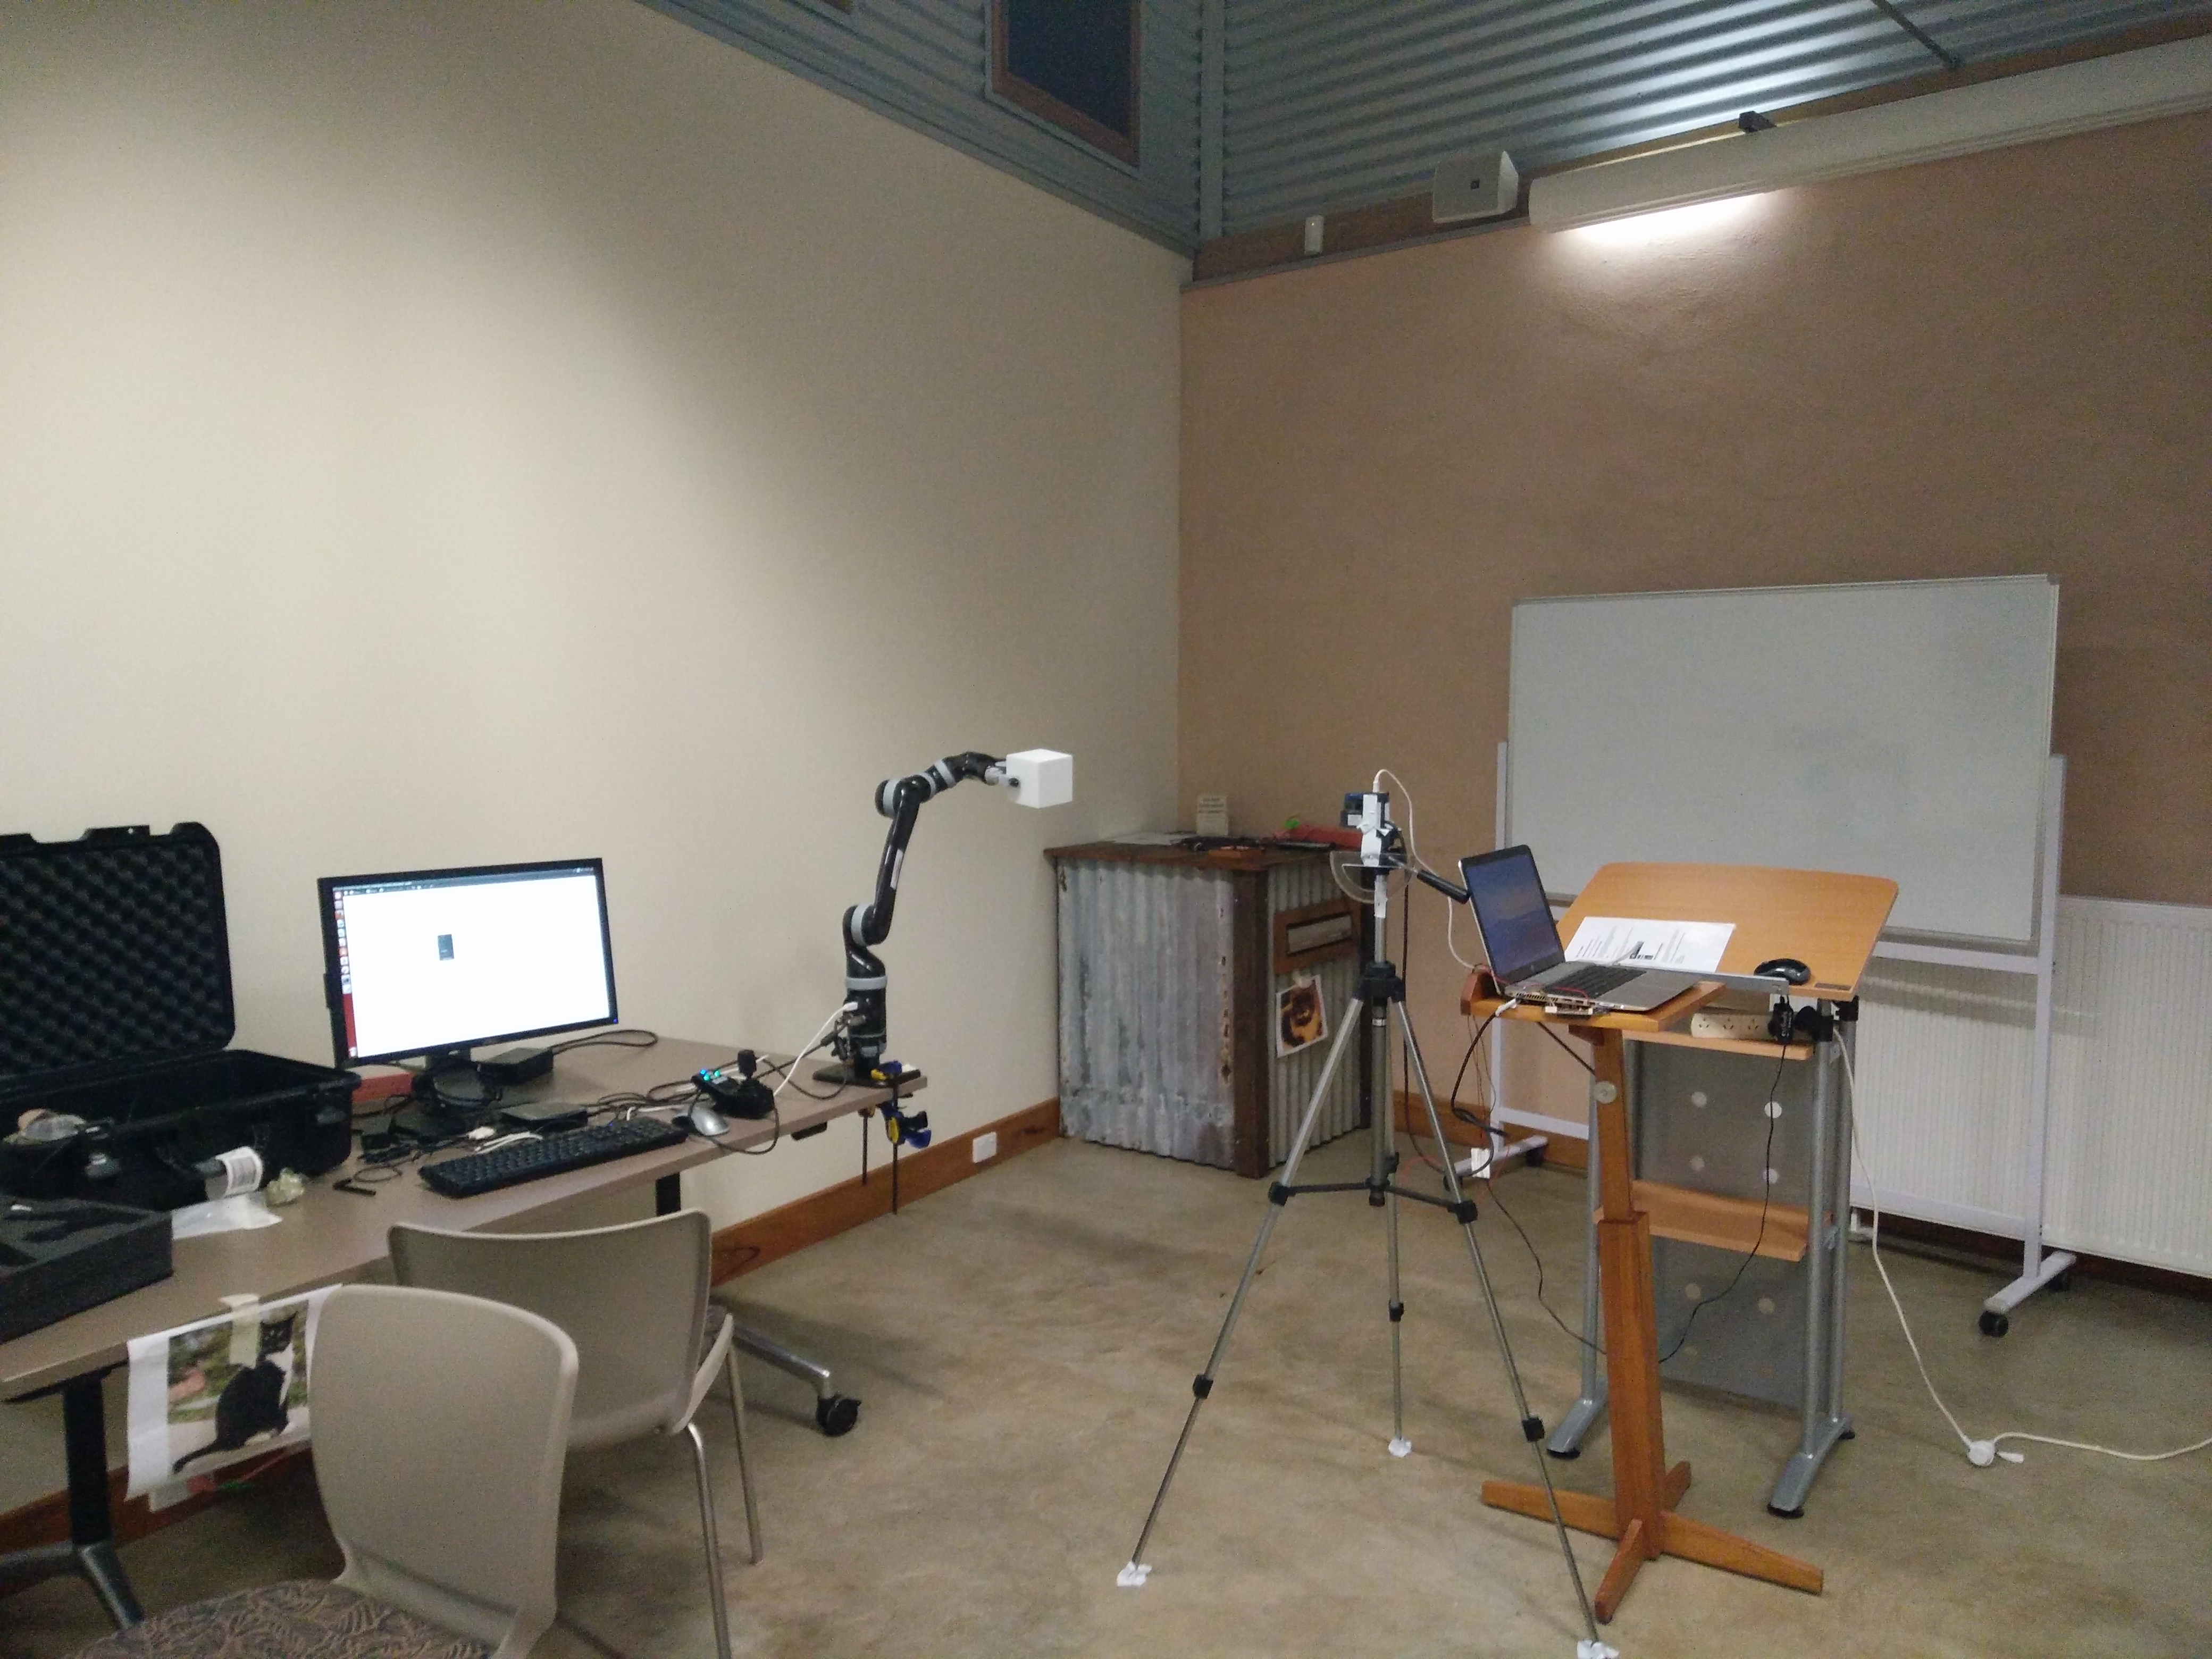
\includegraphics[width=1\textwidth,trim = 0mm 0mm 0mm 0mm,clip=true]{./Figures/experimental_data}\vspace*{0ex}
	  	\caption{setup to measure noise} \label{fig:experimental_data}
\end{figure}

\end{appendices}
\end{document}     